\PassOptionsToPackage{unicode=true}{hyperref} % options for packages loaded elsewhere
\PassOptionsToPackage{hyphens}{url}
%
\documentclass[english,man]{apa6}
\usepackage{lmodern}
\usepackage{amssymb,amsmath}
\usepackage{ifxetex,ifluatex}
\usepackage{fixltx2e} % provides \textsubscript
\ifnum 0\ifxetex 1\fi\ifluatex 1\fi=0 % if pdftex
  \usepackage[T1]{fontenc}
  \usepackage[utf8]{inputenc}
  \usepackage{textcomp} % provides euro and other symbols
\else % if luatex or xelatex
  \usepackage{unicode-math}
  \defaultfontfeatures{Ligatures=TeX,Scale=MatchLowercase}
\fi
% use upquote if available, for straight quotes in verbatim environments
\IfFileExists{upquote.sty}{\usepackage{upquote}}{}
% use microtype if available
\IfFileExists{microtype.sty}{%
\usepackage[]{microtype}
\UseMicrotypeSet[protrusion]{basicmath} % disable protrusion for tt fonts
}{}
\IfFileExists{parskip.sty}{%
\usepackage{parskip}
}{% else
\setlength{\parindent}{0pt}
\setlength{\parskip}{6pt plus 2pt minus 1pt}
}
\usepackage{hyperref}
\hypersetup{
            pdftitle={Characterizing North Carolina's Deaf/Hard-of-Hearing Infants and Toddlers: Predictors of Vocabulary, Diagnosis, and Intervention},
            pdfauthor={Erin Campbell1 \& Elika Bergelson1},
            pdfkeywords={keywords},
            pdfborder={0 0 0},
            breaklinks=true}
\urlstyle{same}  % don't use monospace font for urls
\usepackage{graphicx,grffile}
\makeatletter
\def\maxwidth{\ifdim\Gin@nat@width>\linewidth\linewidth\else\Gin@nat@width\fi}
\def\maxheight{\ifdim\Gin@nat@height>\textheight\textheight\else\Gin@nat@height\fi}
\makeatother
% Scale images if necessary, so that they will not overflow the page
% margins by default, and it is still possible to overwrite the defaults
% using explicit options in \includegraphics[width, height, ...]{}
\setkeys{Gin}{width=\maxwidth,height=\maxheight,keepaspectratio}
\setlength{\emergencystretch}{3em}  % prevent overfull lines
\providecommand{\tightlist}{%
  \setlength{\itemsep}{0pt}\setlength{\parskip}{0pt}}
\setcounter{secnumdepth}{0}

% set default figure placement to htbp
\makeatletter
\def\fps@figure{htbp}
\makeatother

% Manuscript styling
\usepackage{upgreek}
\captionsetup{font=singlespacing,justification=justified}

% Table formatting
\usepackage{longtable}
\usepackage{lscape}
% \usepackage[counterclockwise]{rotating}   % Landscape page setup for large tables
\usepackage{multirow}		% Table styling
\usepackage{tabularx}		% Control Column width
\usepackage[flushleft]{threeparttable}	% Allows for three part tables with a specified notes section
\usepackage{threeparttablex}            % Lets threeparttable work with longtable

% Create new environments so endfloat can handle them
% \newenvironment{ltable}
%   {\begin{landscape}\begin{center}\begin{threeparttable}}
%   {\end{threeparttable}\end{center}\end{landscape}}
\newenvironment{lltable}{\begin{landscape}\begin{center}\begin{ThreePartTable}}{\end{ThreePartTable}\end{center}\end{landscape}}

% Enables adjusting longtable caption width to table width
% Solution found at http://golatex.de/longtable-mit-caption-so-breit-wie-die-tabelle-t15767.html
\makeatletter
\newcommand\LastLTentrywidth{1em}
\newlength\longtablewidth
\setlength{\longtablewidth}{1in}
\newcommand{\getlongtablewidth}{\begingroup \ifcsname LT@\roman{LT@tables}\endcsname \global\longtablewidth=0pt \renewcommand{\LT@entry}[2]{\global\advance\longtablewidth by ##2\relax\gdef\LastLTentrywidth{##2}}\@nameuse{LT@\roman{LT@tables}} \fi \endgroup}

% \setlength{\parindent}{0.5in}
% \setlength{\parskip}{0pt plus 0pt minus 0pt}

% \usepackage{etoolbox}
\makeatletter
\patchcmd{\HyOrg@maketitle}
  {\section{\normalfont\normalsize\abstractname}}
  {\section*{\normalfont\normalsize\abstractname}}
  {}{\typeout{Failed to patch abstract.}}
\patchcmd{\HyOrg@maketitle}
  {\section{\protect\normalfont{\@title}}}
  {\section*{\protect\normalfont{\@title}}}
  {}{\typeout{Failed to patch title.}}
\makeatother
\shorttitle{ELSSP}
\keywords{keywords\newline\indent Word count: X}
\DeclareDelayedFloatFlavor{ThreePartTable}{table}
\DeclareDelayedFloatFlavor{lltable}{table}
\DeclareDelayedFloatFlavor*{longtable}{table}
\makeatletter
\renewcommand{\efloat@iwrite}[1]{\immediate\expandafter\protected@write\csname efloat@post#1\endcsname{}}
\makeatother
\usepackage{lineno}

\linenumbers
\usepackage{csquotes}
\ifnum 0\ifxetex 1\fi\ifluatex 1\fi=0 % if pdftex
  \usepackage[shorthands=off,main=english]{babel}
\else
  % load polyglossia as late as possible as it *could* call bidi if RTL lang (e.g. Hebrew or Arabic)
  \usepackage{polyglossia}
  \setmainlanguage[]{english}
\fi

\title{Characterizing North Carolina's Deaf/Hard-of-Hearing Infants and Toddlers: Predictors of Vocabulary, Diagnosis, and Intervention}
\author{Erin Campbell\textsuperscript{1} \& Elika Bergelson\textsuperscript{1}}
\date{}


\affiliation{\vspace{0.5cm}\textsuperscript{1} Duke University}

\begin{document}
\maketitle

\hypertarget{introduction}{%
\section{Introduction}\label{introduction}}

In the United States, 1-2 children are born with hearing loss, per 1,000 births (CDC, 2018). This translates to 114,000 Deaf or Hard of Hearing (DHH) children born in the U.S. per year (Martin, Hamilton, Osterman, \& Driscoll, 2019). Of these 114,000, \textasciitilde{}90\% will be born to hearing parents (Mitchell \& Karchmer, 2004), in a home where spoken language is likely the dominant communication method. Depending on the type and degree of hearing loss and whether the child uses amplification, spoken linguistic input will be partially or totally inaccessible. Some of these children will develop spoken language proficiency within the range of their hearing peers (Geers, Mitchell, Warner-Czyz, Wang, \& Eisenberg, 2017; Verhaert, Willems, Van Kerschaver, \& Desloovere, 2008), but many will face persistent spoken language deficits (Eisenberg, 2007; Luckner \& Cooke, 2010; Moeller, Tomblin, Yoshinaga-Itano, Connor, \& Jerger, 2007; Sarchet et al., 2014), which may later affect reading ability (Kyle \& Harris, 2010) and academic achievement (Karchmer \& Mitchell, 2003; Qi \& Mitchell, 2012).

Despite many excellent studies examining language development in DHH children, there is still a gap in the literature describing and analyzing spoken language development across the full range of children receiving services for hearing loss, with many studies focusing in on specific subgroups (e.g.~children under age X with Y level of hearing loss and Z amplification approach, e.g. Vohr et al., 2008; Yoshinaga-Itano, Sedey, Wiggin, \& Mason, 2018). In what follows, we first summarize the previous literature on predictors of spoken language outcomes in DHH children. We then provide a brief overview of a common vocabulary measure used in the current study, the MacArthur-Bates Communicative Development Inventory (CDI). Finally, we turn to an empirical analysis of early vocabulary in a wide range of young children receiving state services in North Carolina. We have two broad goals in what follows. First, we aim to provide a comprehensive description of a heterogeneous group of young children who receive state services for hearing loss. Second, we aim to connect the intervention approaches and child characteristics of this sample with children's spoken vocabulary\footnote{Despite exciting, increasing, and converging evidence for benefits of early sign language exposure (e.g., Clark et al., 2016, Davidson et al., 2014; Hrastinski \& Wilbur, 2016; Magnuson, 2000; Schick et al., 2007; Spencer, 1993), the majority of DHH children will not be raised in a sign language environment. This is particularly true for North Carolina, which does not have a large community of sign language users, relative to states like Maryland or areas like Washington D.C. or Rochester, NY. For this reason, and because no families in our sample used a full-fledged signed language, we focus on spoken language development.}, with the broader goal of considering the success of early diagnosis and intervention initiatives.

\hypertarget{predictors-of-language-outcomes}{%
\subsection{Predictors of Language Outcomes}\label{predictors-of-language-outcomes}}

Though the literature points towards spoken language delays and deficits for DHH children, this is a highly variable population with highly variable outcomes (Pisoni, Kronenberger, Harris, \& Moberly, 2018). Previous research indicates that gender (Ching et al., 2013; Kiese-Himmel \& Ohlwein, 2002), additional disability (Ching et al., 2013; Verhaert et al., 2008; Yoshinaga-Itano, Sedey, Wiggin, \& Chung, 2017), degree and configuration of hearing loss (Ching et al., 2013; de Diego-Lázaro, Restrepo, Sedey, \& Yoshinaga-Itano, 2018; Vohr et al., 2011; Yoshinaga-Itano et al., 2017), amplification (Walker et al., 2015), communication (Geers et al., 2017), and early diagnosis/intervention (Yoshinaga-Itano et al., 2017, 2018) predict language outcomes in DHH children. We first provide a brief literature review on the effect of these predictors on language skills in DHH children.

\hypertarget{gender}{%
\subsubsection{Gender}\label{gender}}

For hearing children, the literature points to a female gender advantage in early language acquisition. Girls speak their first word earlier (Macoby, 1966), have a larger (Bornstein, Hahn, \& Haynes, 2004; Fenson et al., 1994; Frank, Braginsky, Yurovsky, \& Marchman, 2017) and faster-growing vocabulary (Huttenlocher, Haight, Bryk, Seltzer, \& Lyons, 1991), and stronger grammatical and phonological skills (Lange, Euler, \& Zaretsky, 2016; Özçalışkan \& Goldin-Meadow, 2010). This finding appears to be consistent across studies (Wallentin, 2009), various spoken languages (Frank, Braginsky, Marchman, \& Yurovsky, 2019), and gesture (Özçalışkan \& Goldin-Meadow, 2010).

The DHH literature presents a more mixed (though rather understudied) picture. On one hand, DHH girls, like hearing girls, have been found to have a larger spoken vocabulary than DHH boys (Ching et al., 2013; Kiese-Himmel \& Ohlwein, 2002). However, in contrast to their hearing peers, DHH children do not seem to show a gender-based difference for some aspects of syntactic development (Pahlavannezhad \& Tayarani Niknezhad, 2014).

\hypertarget{comorbidities}{%
\subsubsection{Comorbidities}\label{comorbidities}}

Additional co-morbid disabilities occur frequently in the DHH population, perhaps as much as three times more than in the hearing population (Pollack, 1997). Incidence estimates for co-occurring disabilities in DHH children range from 25-51\% (Bruce \& Borders, 2015; Guardino, 2008; Holden-Pitt \& Diaz, 1998; Luckner \& Carter, 2001; Picard, 2004; Schildroth \& Hotto, 1996; Soukup \& Feinstein, 2007), with approximately 8\% of DHH children living with 2 or more co-occurring disabilities (Schildroth \& Hotto, 1996).

Some of these conditions, particularly those which carry risk of developmental delay (e.g., Down syndrome), result in language delays independent of hearing loss (Chapman, 1997; Kristoffersen, 2008; Weismer, Lord, \& Esler, 2010). These effects vary by the nature of the specific disability (Cupples et al., 2014, 2018), with cognitive ability more predictive of language outcomes than presence or absence of additional disability (Meinzen-Derr, Wiley, Grether, \& Choo, 2011; Sarant, Holt, Dowell, Richards, \& Blamey, 2008). Disability and hearing loss likely each contribute to a given child's spoken language development (Ching et al., 2013; Rajput, Brown, \& Bamiou, 2003; Van Nierop et al., 2016), with differential effects of each (Vesseur et al., 2016). In some cases, additional disabilities appear to interact with hearing loss to intensify developmental delays (Birman, Elliott, \& Gibson, 2012; Pierson et al., 2007).

Furthermore, incidence of hearing loss is higher among children born premature (defined as \textless{} 37 weeks gestational age). Compared to an incidence of 0.2\% in full-term infants, incidence of hearing loss in extremely premature infants (defined as \textless{} 33 weeks gestational age) ranges 2--11\%, with increased prematurity associated with increased rates of hearing loss (Wroblewska-Seniuk, Greczka, Dabrowski, Szyfter-Harris, \& Mazela, 2017).

Independently of hearing status, prematurity is linked to increased risk of language delay and disorder (Barre, Morgan, Doyle, \& Anderson, 2011; Carter \& Msall, 2017; Cusson, 2003; Rechia, Oliveira, Crestani, Biaggio, \& de Souza, 2016; Van Noort-van Der Spek, Franken, \& Weisglas-Kuperus, 2012; Vohr, 2014). Unfortunately, research on language development in premature DHH children is scant (Vohr, 2016), so it remains unclear how hearing loss and prematurity may interact within spoken language skills. One study of premature infants finds that auditory brainstem response during newborn hearing screening (NBHS) predicts language performance on the PLS-4 at age 3 (Amin, Vogler-Elias, Orlando, \& Wang, 2014), suggesting a link between prematurity, hearing loss, and language development in early childhood, though further research is needed in this domain. In extremely premature DHH children, incidence of additional disabilities may be as high as 73\% (Robertson, Howarth, Bork, \& Dinu, 2009). Indeed, pre-term infants with comorbidities have been found to be more likely to also have hearing loss than those without comorbidities (Schmidt et al., 2003), further complicating language development for this population.

\hypertarget{audiological-characteristics}{%
\subsubsection{Audiological Characteristics}\label{audiological-characteristics}}

Hearing loss varies in severity, ranging from slight to profound (Clark, 1981). More severe hearing loss (less access to spoken language) typically results in more difficulty with spoken language in infancy (Vohr et al., 2008), early childhood (Ching et al., 2010, 2013; Sarant et al., 2008; Sininger, Grimes, \& Christensen, 2010; Tomblin et al., 2015) and school-age children (Wake, Hughes, Poulakis, Collins, \& Rickards, 2004). Although profound hearing loss is associated with more pronounced spoken language difficulty, even mild to moderate hearing loss is associated with elevated risk of language disorders (Blair, Peterson, \& Viehweg, 1985; Delage \& Tuller, 2007).

Hearing loss also varies in whether it affects one ear or both. Bilateral hearing assists speech perception, sound localization, and loudness perception in quiet and noisy environments (Ching, Van Wanrooy, \& Dillon, 2007). The literature on hearing aids and cochlear implants also points to benefits for bilateral auditory input (Lovett, Kitterick, Hewitt, \& Summerfield, 2010; Sarant, Harris, Bennet, \& Bant, 2014; Smulders et al., 2016). At school-age, 3--6\% of children have unilateral hearing loss (Ross, Visser, Holstrum, Qin, \& Kenneson, 2010). Although children with unilateral hearing loss have one \enquote{good ear,} even mild unilateral hearing loss has been tied to higher risk of language delays and educational challenges relative to hearing children (Kiese-Himmel, 2002; Lieu, 2004, 2013; Lieu, Tye-Murray, \& Fu, 2012; Vila \& Lieu, 2015). Just as in the bilateral case, more severe hearing loss leads to greater deficits in spoken language and educational outcomes for children with unilateral hearing loss (Anne, Lieu, \& Cohen, 2017; Lieu, 2013).

Many DHH children receive hearing aids (HAs) or cochlear implants (CIs) to boost access to the aural world. These devices have been associated with better speech perception and spoken language outcomes (Niparko et al., 2010; Walker et al., 2015; Waltzman et al., 1997). In turn, aided audibility predicts lexical abilities in children with HAs (Stiles, Bentler, \& McGregor, 2012).

For both hearing aids and cochlear implants, earlier fit leads to better spoken language skills, if the amplification is effective. For hearing aids, some studies find that children with milder hearing loss who receive hearing aids earlier have better early language achievement than children who are fit with hearing aids later (Tomblin et al., 2015), but this finding does not hold for children with severe-to-profound hearing loss (Kiese-Himmel, 2002; Watkin et al., 2007) (for whom hearing aids are generally ineffective). Analogously, children who are eligible and receive cochlear implants earlier have better speech perception and spoken language outcomes than those implanted later (Artières, Vieu, Mondain, Uziel, \& Venail, 2009; Dettman, Pinder, Briggs, Dowell, \& Leigh, 2007; Miyamoto, Hay-McCutcheon, Kirk, Houston, \& Bergeson-Dana, 2008; Svirsky, Teoh, \& Neuburger, 2004; Yoshinaga-Itano et al., 2018), with best outcomes for children receiving implants before their first birthday (Dettman et al., 2007).

\hypertarget{communication}{%
\subsubsection{Communication}\label{communication}}

Total Communication refers to communication that combines speech, gesture, and elements of sign, sometimes simultaneously. Total communication, while often including elements of sign such as individual signs, is not a full-fledged sign language like American Sign Language (Mueller, 2013; Scott \& Henner, 2020). Clinicians currently employ total communication as an alternative or augmentative communication method for children with a wide range of disabilities (Branson \& Demchak, 2009; Gibbs \& Carswell, 1991; Mirenda, 2003).

Compared to total communication, DHH children using an exclusively oral approach have better speech intelligibility (Dillon, Burkholder, Cleary, \& Pisoni, 2004; Geers et al., 2017; Geers, Spehar, \& Sedey, 2002; Hodges, Dolan Ash, Balkany, Schloffman, \& Butts, 1999) and auditory perception (Geers et al., 2017; O'Donoghue, Nikolopoulos, \& Archbold, 2000). That said, there is some debate as to whether an oral approach facilitates higher spoken language performance, or whether children who demonstrate aptitude for spoken language are steered towards the oral approach rather than total communication (Hall, Levin, \& Anderson, 2017).

\hypertarget{guidelines}{%
\subsubsection{1-3-6 Guidelines}\label{guidelines}}

Early identification (Apuzzo \& Yoshinaga-Itano, 1995; Kennedy et al., 2006; Robinshaw, 1995; White \& White, 1987; Yoshinaga-Itano, Sedey, Coulter, \& Mehl, 1998; Yoshinaga-Itano et al., 2018) and timely enrollment in early intervention programs (Ching, Dillon, Leigh, \& Cupples, 2018; Ching et al., 2013; Holzinger, Fellinger, \& Beitel, 2011; Vohr et al., 2008, 2011; Watkin et al., 2007) are associated with better language proficiency. Indeed, DHH children who receive prompt diagnosis and early access to services have been found to meet age-appropriate developmental outcomes, including language (Stika et al., 2015).
In line with these findings, the American Academy of Pediatricians (AAP) has set an initiative for Early Hearing Detection and Intervention (EHDI). Their EHDI guidelines recommend that DHH children are screened by 1 month old, diagnosed by 3 months old, and enter early intervention services by 6 months old. We refer to this guideline as 1-3-6. Meeting this standard appears to improve spoken language outcomes for children with HL (Yoshinaga-Itano et al., 2017, 2018) and the benefits appear consistent across a range of demographic characteristics.

At a federal level in the U.S., the Early Hearing Detection and Intervention Act of 2010 (Capps, 2009) was passed to develop state-wide systems for screening, evaluation, diagnosis, and \enquote{appropriate education, audiological, medical interventions for children identified with hearing loss,} but policies for early diagnosis and intervention vary by state. As of 2011, 36 states (including North Carolina; ``15A NCAC 21F .1201 - .1204,'' 2000) mandate universal newborn hearing screening (UNHS; National Conference of State Legislatures, 2011). All states have some form of early intervention programs that children with hearing loss can access (NAD, n.d.), but the specifics vary state-by-state. For instance, half of the states in the US do not consider mild hearing loss an eligibility criterion for early intervention (Holstrum, Gaffney, Gravel, Oyler, \& Ross, 2008); North Carolina does include mild hearing loss in early intervention.

In evaluating the success of this initiative, the AAP (EHDI, n.d.) finds that about 70\% of US children who fail their newborn hearing screening test are diagnosed with hearing loss before 3 months old, and that 67\% of those diagnosed (46\% of those that fail newborn hearing screening) begin early intervention services by 6 months old. These findings suggest that there are breaks in the chain from screening to diagnosis and from diagnosis to intervention, with potential ramifications for the language development of children not meeting these guidelines. We return to this in the discussion.

\hypertarget{quantifying-vocabulary-growth-in-dhh-children}{%
\subsection{Quantifying vocabulary growth in DHH children}\label{quantifying-vocabulary-growth-in-dhh-children}}

In what follows, we analyze data from the MacArthur Bates Communicative Development Inventory (CDI, Fenson et al., 1994). This parent-report instrument gathers information about children's vocabulary development, and is commonly used in both research and applied settings. The Words and Gestures version of the form is normed for 8--18-month-olds. On Words and Gestures, parents indicate whether their child understands and/or produces each of the 398 vocabulary items, and answer questions about young children's early communicative milestones. The Words and Sentences version of the form is normed for 16-30-month-olds. On Words and Sentences, parents indicate whether their child produces each of the 680 vocabulary items, and answer some questions about grammatical development. The CDI has been normed on a large set of participants across many languages (Anderson \& Reilly, 2002; Frank et al., 2017; Jackson-Maldonado et al., 2003).

The CDI has also been validated for DHH children with cochlear implants (Thal, Desjardin, \& Eisenberg, 2007). More specifically, in this validation, researchers asked parents to complete the CDI, administered the Reynell Developmental Language Scales, and collected a spontaneous speech sample. All comparisons between the CDI and the other measures yielded significant correlations ranging from 0.58 to 0.93. Critically, the children in this study were above the normed age range for the CDI, and thus this validation helps to confirm that the CDI is a valid measurement tool for older DHH children. In further work, Castellanos, Pisoni, Kronenberger, and Beer (2016) find that in children with CIs, number of words produced on the CDI predicts language, executive function, and academic skills up to 16 years later. Building on this work, several studies have used the CDI to measure vocabulary development in DHH children (Yoshinaga-Itano et al. (2017); Yoshinaga-Itano et al. (2018); de Diego-Lázaro et al. (2018); Vohr et al. (2008); Vohr et al. (2011); summarized in Table \ref{tab:CDIsummary}). We build on this literature in our analyses below.

\begin{table}

\caption{\label{tab:CDIsummary}Summary of findings of CDI studies in DHH children}
\centering
\resizebox{\linewidth}{!}{
\begin{tabular}[t]{l|l|l|l|l|l|l|l|l}
\hline
Study & Population & Gender & 1-3-6 & Laterality & Degree & Amplification & Communication & Comorbidities\\
\hline
Yoshinaga-Itano et al., 2017 & 8-39 month children with bilateral hearing loss & No effect & 1-3-6 + & Did not study & More severe - & Did not study & Did not study & Comorbidities -\\
\hline
Yoshinaga-Itano et al., 2018 & Children with cochlear implants & Did not study & 1-3-6 + & Did not study & Did not study & Earlier CI activation + & Did not study & Did not study\\
\hline
De Diego-Lazaro et al., 2018 & Spanish speaking children with bilateral hearing loss & No effect & Earlier intervention + & Did not study & Milder + & More functional hearing + & Did not study & Did not study\\
\hline
Vohr et al., 2011 & 18-24 month olds with hearing loss & Did not study & Earlier intervention + & Did not study & Milder + & Did not study & Did not study & NICU stay -; Comorbidities -\\
\hline
\multicolumn{9}{l}{\textsuperscript{a} + equals bigger vocab, - equals smaller vocab}\\
\end{tabular}}
\end{table}

\hypertarget{goals-and-predictions}{%
\subsection{Goals and Predictions}\label{goals-and-predictions}}

This study aims to 1) characterize the demographic, audiological, and intervention variability in the population of DHH children receiving state services for hearing loss; 2) identify predictors of vocabulary delays; and 3) evaluate the success of early identification and intervention efforts at a state level. We include three subgroups of DHH children traditionally excluded from studies of language development: children with additional disabilities, children with unilateral hearing loss, and children from bilingual or non-English-speaking households (e.g., Yoshinaga-Itano et al., 2018; Nicholas \& Geers, 2006).

For the first goal, we had reason to expect that many of these variables would be related, due to known causal relations (e.g., cochlear implants recommended for severe hearing loss, but not mild hearing loss). We sought to provide descriptive documentation about the distrubution of demographic, audiological, and intervention characteristics in a diverse sample of DHH children receiving state services. For the second, we hypothesized that male gender, more severe degree of hearing loss, bilateral hearing loss, no amplification use, premature birth, and presence of additional disabilities would predict larger spoken vocabulary delay than female gender, less severe degree of hearing loss, unilateral hearing loss, amplification use, full term birth, and lack of additional disabilities, respectively. We did not have strong predictions regarding the effects of communication method or presence of other health issues (e.g., congenital heart malformation) on vocabulary. For the third goal, based on the prior literatal summarized above, we hypothesized that children with less residual hearing (i.e., bilateral, more severe) and no co-occurring conditions would be earlier diagnosed and earlier to begin language services, and that earlier diagnosis would predict earlier intervention.

\hypertarget{methods}{%
\section{Methods}\label{methods}}

Clinical evaluations were obtained through an ongoing collaboration with the North Carolina Early Language Sensory Support Program (ELSSP), an early intervention program serving children with sensory impairments from birth to 36 months. ELSSP passed along deidentified evaluations to our team after obtaining consent to do so from each family. No eligibility criteria beyond hearing loss and receiving an ELSSP evaluation were imposed, given our goal of characterizing the full range of DHH children with hearing loss in North Carolina.

The clinical evaluations included demographic and audiological information, CDI vocabulary scores, and the results of any clinical assessments administered (e.g., PPVT), detailed further below. For some children (n=47), multiple evaluations were available from different timepoints. In these cases, only the first evaluation was considered for this study, due to concerns regarding within-subjects variance for statistical analysis.

While this collaboration is ongoing, we opted to pause for this analysis upon receiving data from 100 children. Thus, the reported sample below consists of 100 children (56 male / 44 female) ages 4.20--36.17 months (M=21.21, SD=9.08). Race and socioeconomic information were not available. Families were administered either the Words and Gestures or Words and Sentences version of the CDI based on clinician judgement. Children who were too old for Words and Gestures, but who were not producing many words at the time of assessment, were often given Words and Gestures (n=37). Families for whom Spanish was the primary language (n=14) completed the Spanish language version of the CDI (Jackson-Maldonado et al., 2003).

\begin{table}

\caption{\label{tab:CDIinfo}CDI details}
\centering
\resizebox{\linewidth}{!}{
\begin{tabular}[t]{l|l|l|l|l}
\hline
CDI version & Average Age (SD) & Average Comprehension (SD) & Average Production (SD) & \% Developmental Delays\\
\hline
WG (n=74) & 20.05 (8.82) months & 105 (99.7) words & 32 (53.4) words & 18.92\%\\
\hline
WS (n=24) & 26.03 (7.78) months & NA & 149 (180.1) words & 4.17\%\\
\hline
\end{tabular}}
\end{table}

\begin{longtable}[t]{l|l|r}
\caption{\label{tab:comorbid-info}Additional Diagnoses (n=39)}\\
\hline
Condition & Specific Condition & n\\
\hline
Premature &  & 17\\
\hline
 & Extremely Premature & 11\\
\hline
 & NICU stay & 16\\
\hline
Health Issues &  & 36\\
\hline
 & Heart & 9\\
\hline
 & Lung & 5\\
\hline
 & Illness & 15\\
\hline
 & Feeding Issues & 14\\
\hline
 & Pregnancy/Birth Complications & 11\\
\hline
 & Musculoskeletal & 9\\
\hline
 & Cleft Lip/Palate & 4\\
\hline
 & Other & 15\\
\hline
Developmental Concerns &  & 17\\
\hline
 & Down Syndrome & 5\\
\hline
 & Chromosomal Issues & 2\\
\hline
 & Neural Tube Defects & 2\\
\hline
 & Other & 10\\
\hline
Vision Loss &  & 5\\
\hline
 & Retinopathy of Prematurity & 1\\
\hline
 & Nearsightedness & 1\\
\hline
 & Farsightedness & 1\\
\hline
 & Cortical Visual Impairment & 1\\
\hline
\end{longtable}

With regard to comorbid diagnoses, children in this sample were coded as yes/no for cognitive development concerns (e.g., Down syndrome, global developmental delays; Cornelia de Lange syndrome), yes/no for premature birth (i.e., more than 3 weeks premature), yes/no for health issues (e.g., heart defects, kidney malformations, VACTERL association), and yes/no for vision loss (not corrected to normal by surgery or glasses); see Table \ref{tab:comorbid-info}.

\begin{table}[!h]

\caption{\label{tab:amp-info}Audiological Characteristics of the Sample}
\centering
\resizebox{\linewidth}{!}{
\begin{tabular}[t]{l|l|r|r|r|r}
\hline
Laterality & Amplification & mean\_HLbetter & mean\_HLworse & mean\_age\_amplification & mean\_age\_implantation\\
\hline
Bilateral & CI & 85.60 & 89.79 & 11.29 & 14.12\\
\hline
Bilateral & HA & 47.02 & 55.57 & 8.28 & NaN\\
\hline
Bilateral & none & 49.67 & 53.65 & NaN & NaN\\
\hline
Unilateral & HA & 4.70 & 56.04 & 10.91 & NaN\\
\hline
Unilateral & none & 2.50 & 73.90 & 8.50 & NaN\\
\hline
\end{tabular}}
\end{table}

Degree of hearing loss was most often reported with a written description (e.g., \enquote{mild sloping to moderate} or \enquote{profound high frequency loss}). We created 3 variables: hearing loss in the better ear, hearing loss in the worse ear, and average hearing loss (average of better and worse ear). For the analyses below, we primarily use hearing loss in the worse ear to avoid any redundancies with laterality. Using the ASHA hearing loss guidelines, each of these hearing loss measures was coded with the decibels of hearing loss (dB HL) corresponding with the median dB HL for the level of hearing loss (e.g., moderate hearing loss was coded as 48 dB HL), and sloping hearing loss was coded as the average of the levels (e.g.~mild to moderate was coded as 40.5 dB HL). Participants were also coded for unilateral or bilateral hearing loss; presence or absence of Auditory Neuropathy Spectrum Disorder; and etiology of hearing loss (sensorineural, conductive, or mixed). Amplification was recorded as the device the child used at the time of assessment: either hearing aid, cochlear implant, or none. See Table \ref{tab:amp-info} for audiological characteristics of the sample.

\begin{table}[!h]

\caption{\label{tab:comm-info}Language and communication characteristics of the sample}
\centering
\begin{tabular}[t]{l|r|r|r|r}
\hline
Communication & English & Hindi & Spanish & Total\\
\hline
cued speech & 1 & 0 & 0 & 1\\
\hline
spoken & 68 & 1 & 10 & 79\\
\hline
total communication & 15 & 0 & 3 & 18\\
\hline
\end{tabular}
\end{table}

Communication method was recorded as spoken language, total communication, or cued speech. One participant had a parent fluent in sign language, but the reported communication method in the home was total communication. No child in our sample used American Sign Language or another signed language. The forms also listed the primary language spoken at home, which we binned into English-speaking and non-English-speaking. 85\% of families spoke English, and 14\% spoke Spanish. For one child, who was adopted from a non-English-speaking country after their second birthday, we recorded the language background as non-English-speaking, although the child's adoptive parents are English-speaking, because the child had lived most of her life in a non-English-speaking environment. Language and communication information is summarized in Table \ref{tab:comm-info}.

\begin{table}[!h]

\caption{\label{tab:meets136-info}Meets 1-3-6 table}
\centering
\begin{tabular}[t]{l|l}
\hline
 & \\
\hline
Diagnosis by 3 months & 69.47\%\\
\hline
Average Age Diagnosis (SD) & 4.65 (7.19) months\\
\hline
Intervention by 6 months & 39.18\%\\
\hline
Average Age Intervention (SD) & 11.12 (8.54) months\\
\hline
Meets 1-3-6 & 36.84\%\\
\hline
\end{tabular}
\end{table}

Age at screening was measured as the child's age in months at their first hearing screening. Age at screening was available for 68 participants. All participants with a screening age available were screened at birth or while in the NICU. We presume that the vast majority of participants without age at screening received their screening as newborns, as North Carolina boasts a 98\% NBHS rate (NCDHHS, 2013). Age at diagnosis was taken as the age in months when children received their first hearing loss diagnosis. All children were enrolled in birth-to-three early intervention services through ELSSP, and the date of enrollment was listed on the clinician evaluation. For determining whether participants met the 1-3-6 guidelines, given the very high rates of early screening reported in our sample and by the state, we imputed missing data by assuming that children met the \enquote{screening by 1 month} criterion if they met the \enquote{diagnoses by 3 months} and \enquote{service enrollment by 6 months} criteria; see Table \ref{tab:meets136-info}. Finally, we also calculated the number of hours of early intervention services received per month (including service coordination, speech therapy, and occupational therapy, among others) based on the clinician report.

\begin{table}

\caption{\label{tab:variables-list}Variables table}
\centering
\resizebox{\linewidth}{!}{
\begin{tabular}[t]{l|l|l}
\hline
Variable & Scale & Range\\
\hline
Age & Continuous & 4.2-36 months (mean (SD): 21 (9.1))\\
\hline
Age at Amplification & Continuous & 2-30 months (mean (SD): 9 (6.7))\\
\hline
Age at Diagnosis & Continuous & 0-30 months (mean (SD): 5 (7.2))\\
\hline
Age at Implantation & Continuous & 7-32 months (mean (SD): 14 (7.2))\\
\hline
Age at Intervention & Continuous & 1-33 months (mean (SD): 11 (8.5))\\
\hline
Amplification & Categorical & Hearing Aid / Cochlear Implant / None\\
\hline
Communication & Categorical & Spoken / Total Communication / Cued Speech\\
\hline
Degree Hearing Loss (worse ear) & Continuous & 17.75-100 dB HL (mean (SD): 64 (24))\\
\hline
Developmental Delay & Categorical & Yes / No\\
\hline
Gender & Categorical & Female / Male\\
\hline
Health Issues & Categorical & Yes / No\\
\hline
Language in Home & Categorical & English / Other\\
\hline
Laterality & Categorical & Unilateral / Bilateral\\
\hline
1-3-6 & Categorical & Yes / No\\
\hline
Premature Birth & Categorical & Full-term / Premature\\
\hline
Services Per Month & Continuous & 0-43 services per month (mean (SD): 6 (6.4))\\
\hline
Etiology & Categorical & Sensorineural / Conductive / Mixed\\
\hline
CDI - Words Produced & Continuous & 0-635 words (mean (SD): 61 (111.2))\\
\hline
\end{tabular}}
\end{table}

\hypertarget{results}{%
\section{Results}\label{results}}

We split the results into three parts. In the first, we explore relationships among child demographic, audiological, and clinical variables. In the second, we use these variables to predict vocabulary development. Finally, in the third, we describe the implementation of the EHDI 1-3-6 guidelines and predictors of early diagnosis and intervention in this sample. All analyses were conducted in R. All code is available on Github.

\hypertarget{part-i-interactions-among-variables}{%
\subsection{Part I: Interactions Among Variables}\label{part-i-interactions-among-variables}}

Before we test how these variables may be related to vocabulary, we describe their relationships to each other. As would be expected, many health, audiological, and clinical characteristics are not distributed randomly across this sample of children. To quantify this statistically, we used Bonferroni-corrected chi-square tests between each of our variables (gender (male/female), laterality (bi-/uni-lateral hearing loss), health issues (yes/no), developmental delays (yes/no), premature birth (yes/no), language background (English/non-English), 1-3-6 (yes/no), degree of hearing loss (mild, moderate, severe/profound as defined above), etiology (sensorineural/conductive), services received per month (binned into 0-2, 3-6, and \textgreater{}7 - to create maximally evenly sized bins), communication (spoken/total communication) and amplification (hearing aids/cochlear implants/none)). Because the chi-square statistic assumes n \textgreater{} 5 is \emph{expected} in the majority of the cells for each test (preferably \(\geq\) 80\% McHugh, 2013), we excluded mixed hearing loss (n=8) and cued speech (n=1) from this section of the analysis. Strictly speaking, some of these variables are not expected to be randomly distributed relative to each other (e.g., premature birth and health issues; degree and amplification), but quantifying the differences via chi-square using a conservative significance threshold lets us highlight the strongest relationships within this dataset.

Given that we ran 66 Chi-square tests, Bonferroni-corrected alpha for this set of analyses was p \textless{} 0.0007. Of these 66 combinations of variables, p \textless{} .05 for 26, and 9 survived Bonferroni correction. We are only discussing the latter below, but the full set of results can be found in Figure \ref{fig:relationships-plot}.

\begin{figure}
\centering
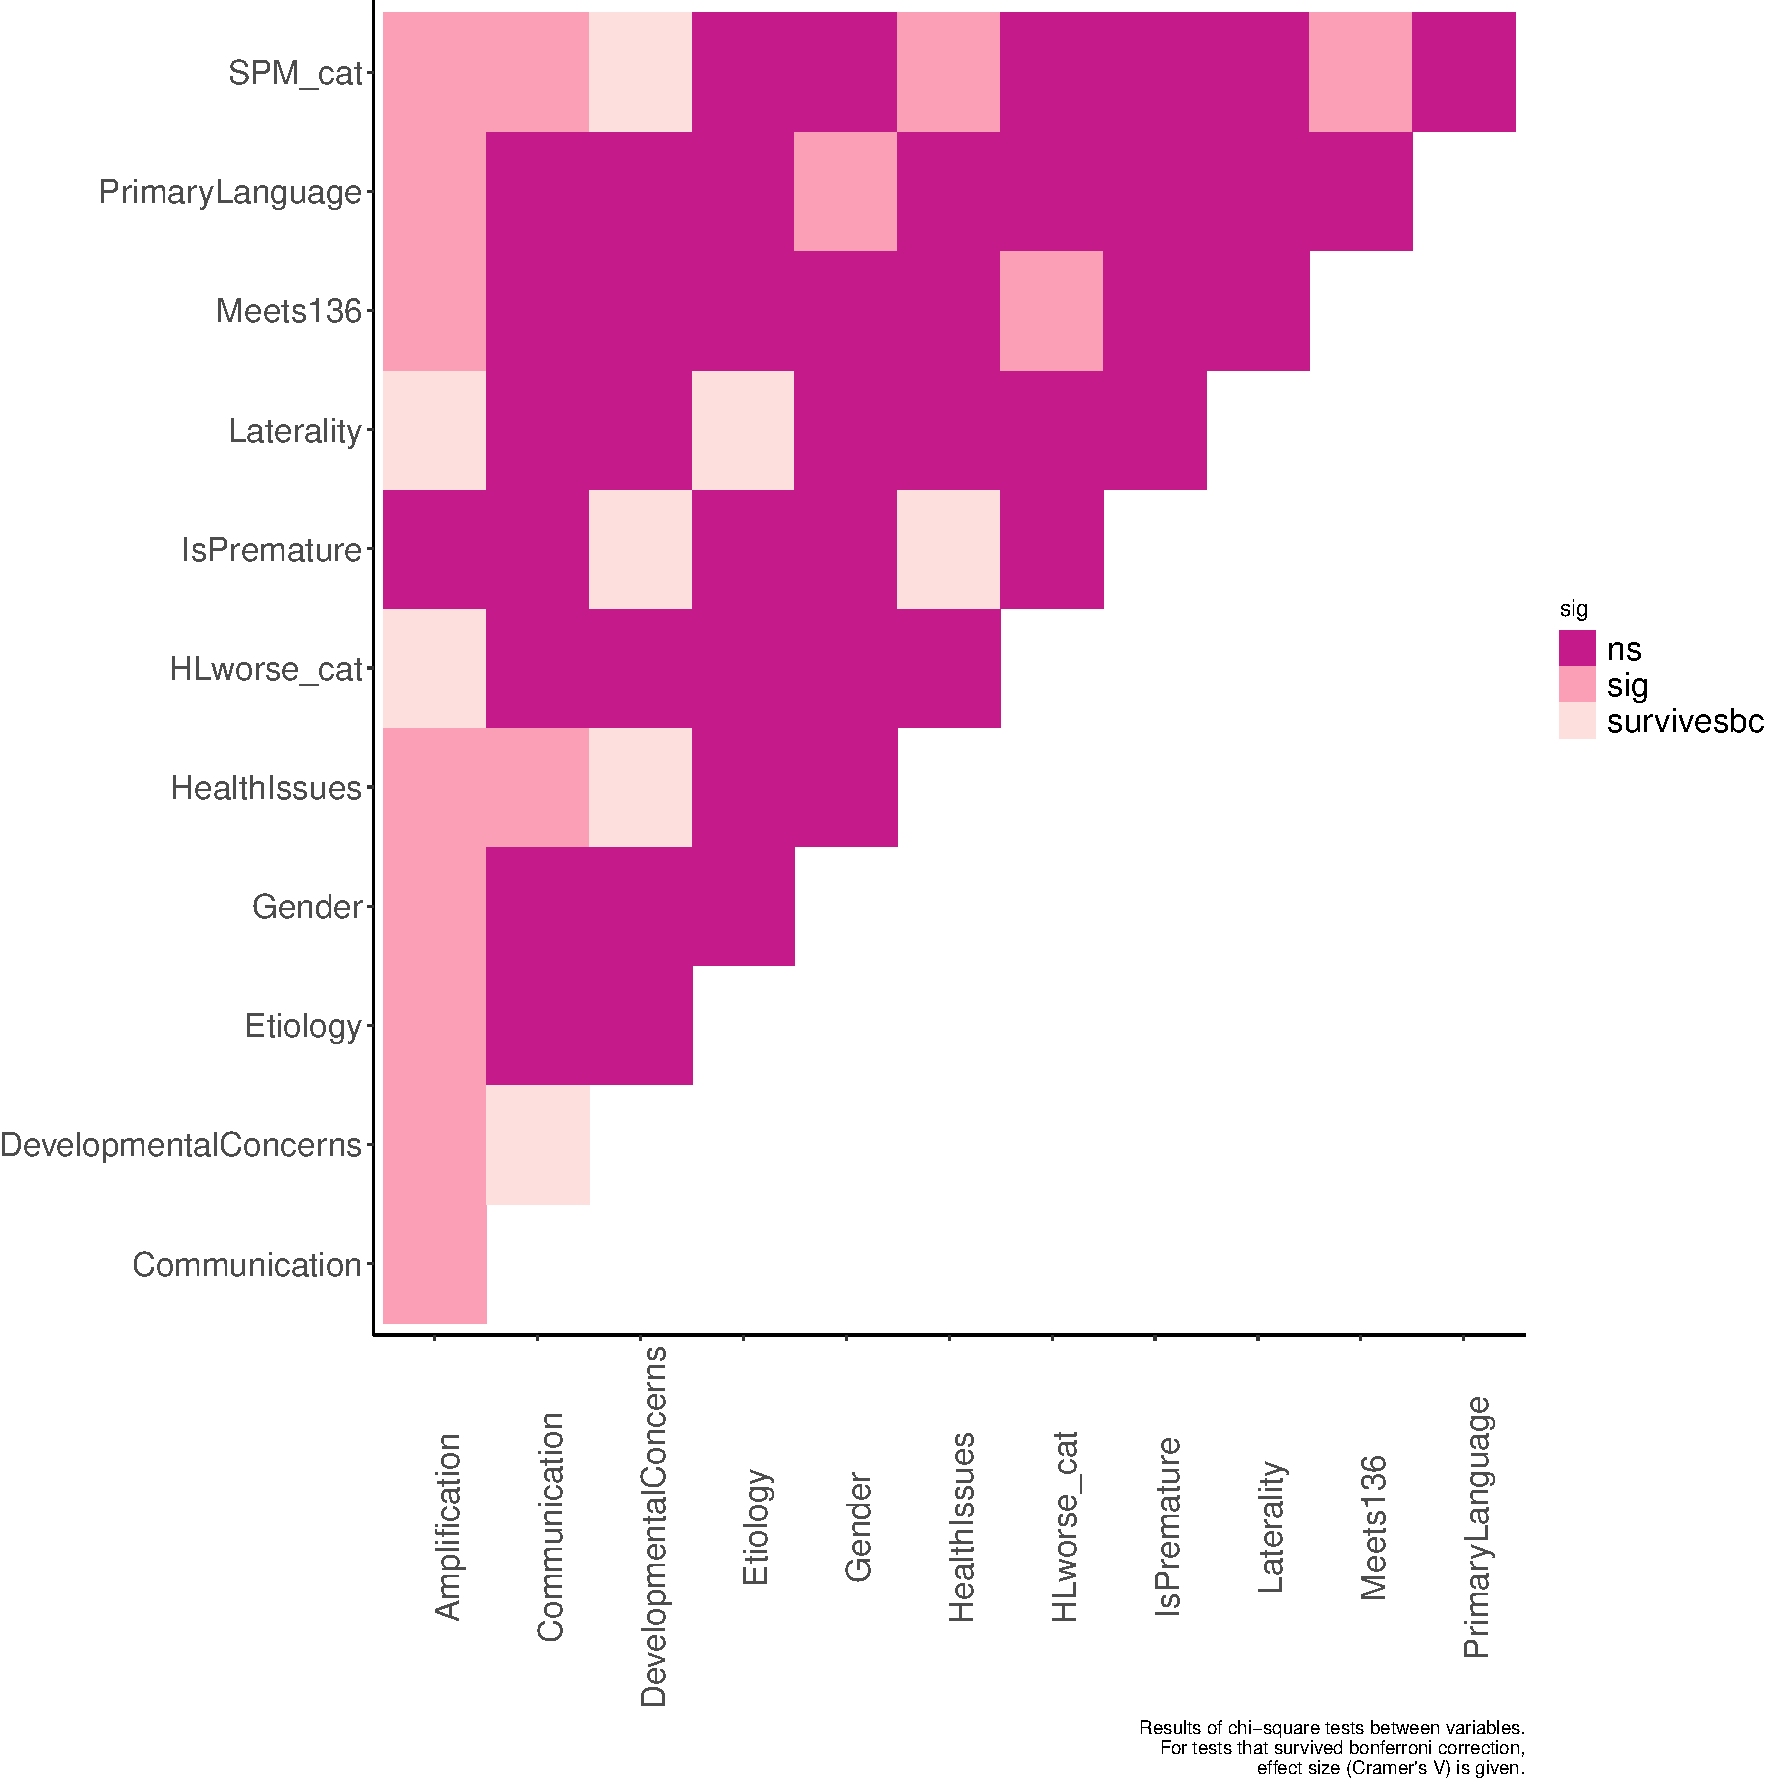
\includegraphics{ELSSP_paper_files/figure-latex/relationships-plot-1.pdf}
\caption{\label{fig:relationships-plot}Results of chi-square tests between variables. For tests that survived Bonferroni correction, effect size (Cramer's V) is given.}
\end{figure}

As expected, we found that health issues, developmental delays, and premature birth were highly interrelated in our sample, such that children born premature were more likely to also experience health issues (\(X^2\) (1, N = 98) = 23.9, p \textless{} .0001) and developmental delays (\(X^2\) (1, N = 98) = 11.63, p = .0006), and children with developmental delays were more likely to also experience health issues (\(X^2\) (1, N = 98) = 20.87, p \textless{} .0001). Children with developmental delays received more services per month than typically-developing children (\(X^2\) (2, N = 95) = 22.17, p \textless{} .0001) and were more likely to use total communication (\(X^2\) (2, N = 98) = 22.51, p \textless{} .0001). Likewise, children who used total communication received more services per month than children using spoken language (\(X^2\) (4, N = 95) = 21.35, p = .0003).

We also confirmed expected relationships among many of the audiological characteristics. There was a significant relationship between laterality and etiology (\(X^2\) (2, N = 88) = 18.29, p = .0001), such that children with conductive hearing loss were more likely to have unilateral hearing loss, and children with sensorineural hearing loss were more likely to have a bilateral loss\footnote{All children with mixed hearing loss (n=8) had bilateral hearing loss.}. Chi-square tests showed that laterality (\(X^2\) (2, N = 98) = 16.43, p = .0003) and degree of hearing loss (\(X^2\) (4, N = 87) = 28.45, p \textless{} .0001) were related to amplification in our sample. Children with bilateral hearing loss were more likely than children with unilateral hearing loss to use a hearing aid or cochlear implant; no child with unilateral hearing loss used a cochlear implant, and many children with unilateral hearing loss used no amplification. Regarding degree, children with severe to profound hearing loss were more likely to use a cochlear implant than children with less severe hearing loss (i.e., mild or moderate).

\hypertarget{part-ii-influence-on-vocabulary}{%
\subsection{Part II: Influence on vocabulary}\label{part-ii-influence-on-vocabulary}}

\begin{figure}
\centering
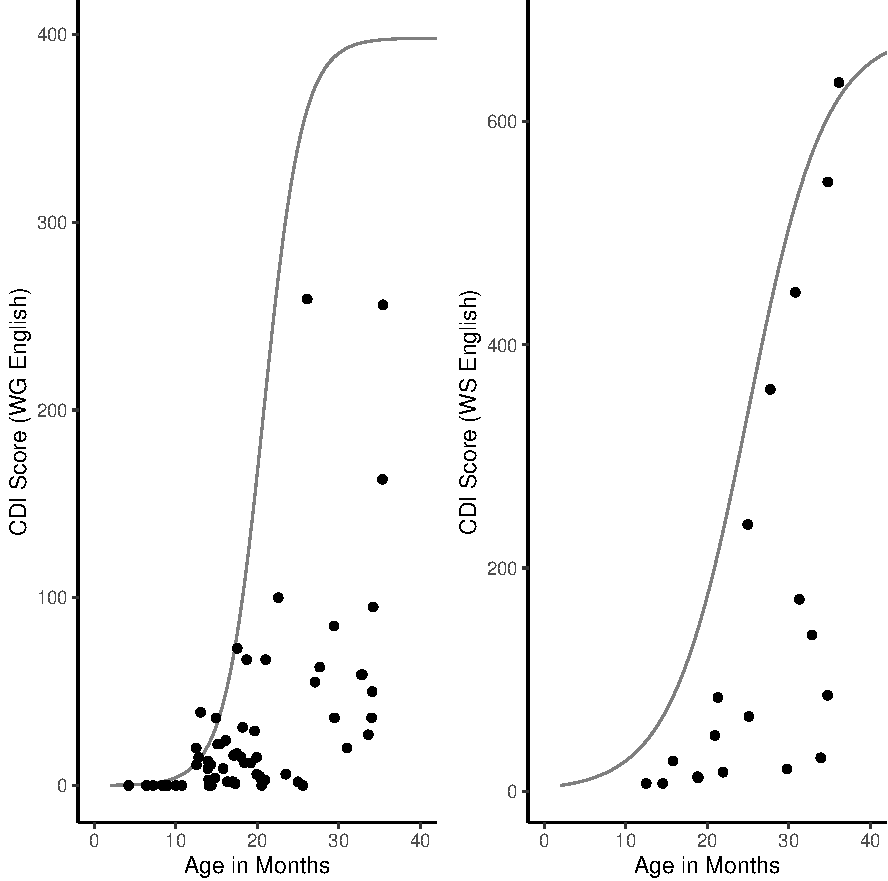
\includegraphics{ELSSP_paper_files/figure-latex/english-curves-1.pdf}
\caption{\label{fig:english-curves}Growth curve from Wordbank American English 50th percentile data. Black triangles show vocabulary scores of individual DHH children.}
\end{figure}

\begin{figure}
\centering
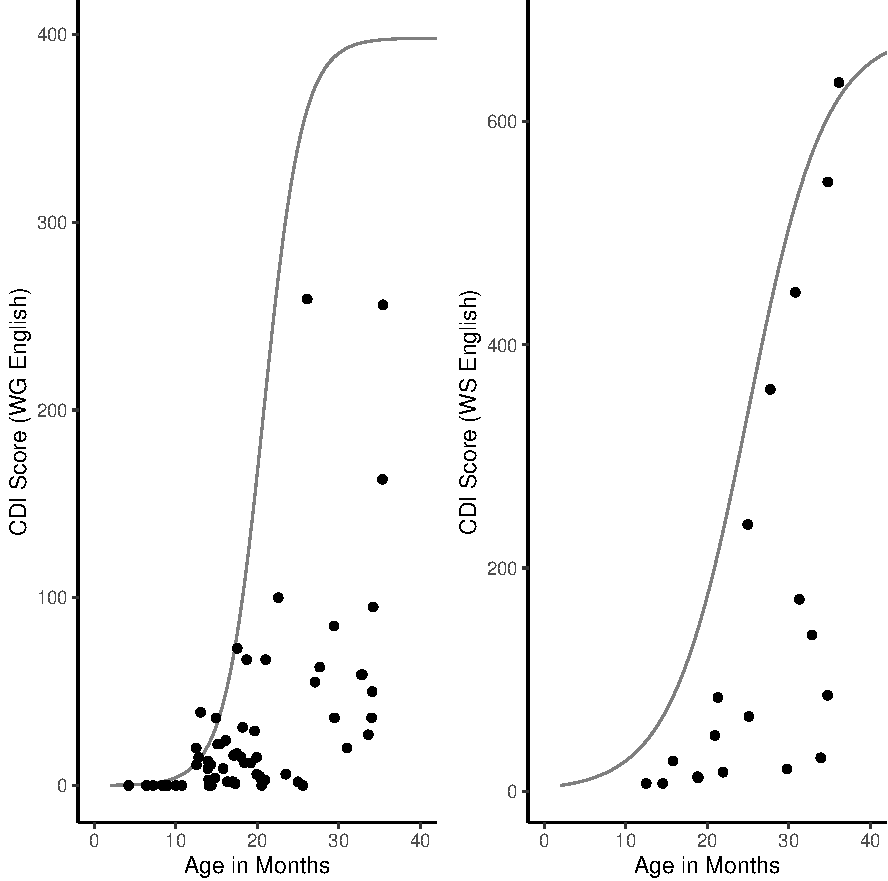
\includegraphics{ELSSP_paper_files/figure-latex/spanish-curves-1.pdf}
\caption{\label{fig:spanish-curves}Growth curve from Wordbank Spanish (Mexican) 50th percentile data. Black triangles show vocabulary scores of individual DHH children.}
\end{figure}

We next turn to the relationship between each of these variables and children's productive vocabulary, as measured by the CDI. Figures \ref{fig:english-curves} \& \ref{fig:spanish-curves} show the vocabulary scores of children in our samples relative to norms for hearing children for English and Spanish respectively. Descriptively, we found widespread vocabulary delays on both Words and Gestures and Words and Sentences, with the majority of DHH children testing around or below the 25th percentile for hearing children (based on WordBank norms; Frank et al., 2017).

As noted above, the CDI is composed of two instruments, which differ in number of questions (i.e.~the maximum vocabulary score is 398 on Words and Gestures and 680 on Words and Sentences; 428 and 680 respectively for Spanish language CDI). To take this into account, rather than using the raw number of words produced as our outcome variable, we use WordBank norms to establish the difference (in months) between the child's chronological age and their predicted age based on their vocabulary, derived from the WordBank norms (Frank et al., 2017). We call this derived variable \emph{vocabulary delay}.

More specifically, to compute a child's predicted age from their vocabulary score, we used the 50th percentile for productive vocabulary from Wordbank data typically-developing infants \footnote{n(WG-English)=1071, n(WG-Spanish)=760, n(WS-English)=1461, n(WS-Spanish)=1092} (Frank et al., 2017) to create binary logistic growth curves separately for the Words and Gestures and Words and Sentences versions of the CDI for American English and Mexican Spanish. For each child, we took the number of words they produced divided by the number of words on the instrument, to give us the proportion of words produced. We used this proportion in an inverse prediction from the binary logistic regression curves to generate a predicted age. That is, for each possible CDI score, the growth curve provided the age that the score would be achieved for the 50th percentile trajectory. Finally, we subtracted the predicted age from each child's chronological age to calculate their vocabulary delay. However, for children producing 0 words, this approach was not appropriate due to the long tails on the growth curves. Thus, for this subset of children, we took the x-intercept from Wordbank (8 months for English, and 9 months for Spanish), and subtracted that value from the child's chronological age to get their vocabulary delay.

To look at the relationship between our predictor variables and CDI scores, we next conducted multiple linear regression, using vocabulary delay as our outcome variable. \footnote{We excluded the adopted child from this section of the analysis due to concerns about comparing her score to the American English CDI norms.}

Our full regression model included all variables: Vocabulary Delay \textasciitilde{} Gender + Developmental Delay + Health Issues + Premature Birth + Laterality + Degree + Amplification + Communication + Meets 1-3-6 + Services Received Per Month + Language Background.

This model accounted for significant variance in vocabulary delay (adjusted-R\textsuperscript{2} = 0.59, \emph{p} \textless{} .001; see Figure \ref{fig:full-delay-betas}). We next performed stepwise model comparison using stepAIC (MASS) to pare down the model. This process selected only the predictors which incrementally improved model fit, measured by Akaike's Information Criterion (AIC), which considers goodness of fit and model complexity (penalizing models with many predictors).

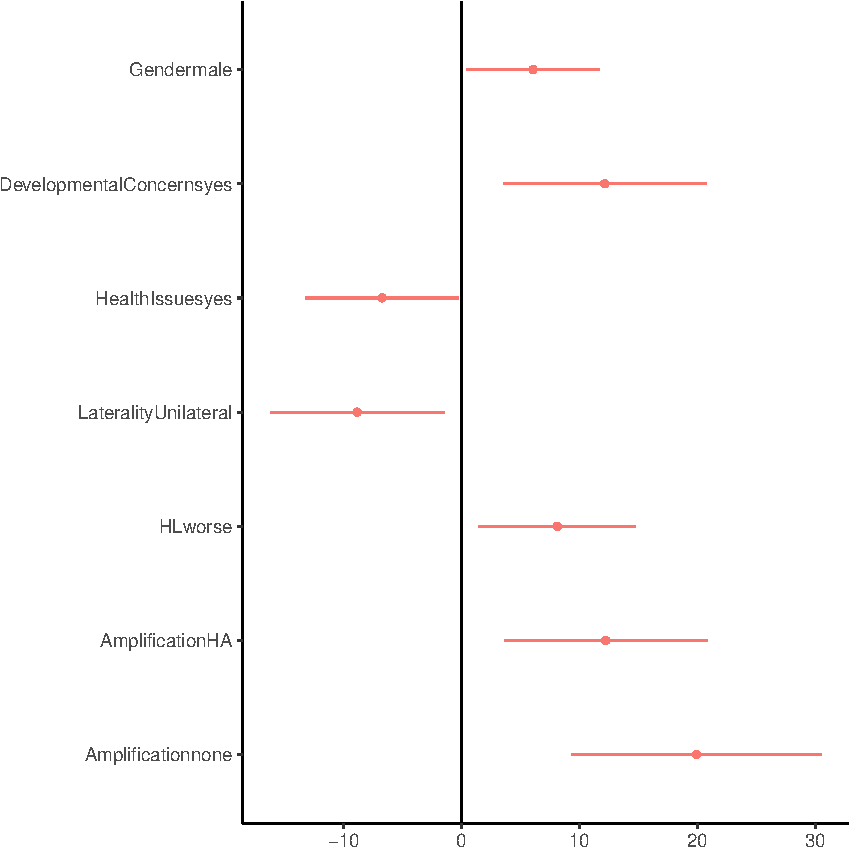
\includegraphics{ELSSP_paper_files/figure-latex/delay-betas-1.pdf}

\begin{table}[H]
\centering
\begin{tabular}{l|r|r|r|r}
\hline
term & estimate & std.error & statistic & p.value\\
\hline
(Intercept) & -0.6088807 & 1.7157582 & -0.3548756 & 0.7235829\\
\hline
LateralityUnilateral & -2.6914102 & 1.1359432 & -2.3693176 & 0.0201422\\
\hline
AmplificationCI & -3.4923095 & 1.4891773 & -2.3451266 & 0.0214079\\
\hline
AmplificationHA & -3.8330674 & 1.1337633 & -3.3808356 & 0.0011037\\
\hline
Age & 0.5522518 & 0.0559563 & 9.8693442 & 0.0000000\\
\hline
\end{tabular}
\end{table}

\begin{table}[H]
\centering
\begin{tabular}{l|r|r}
\hline
  & GVIF & Df\\
\hline
Laterality & 1.178944 & 1\\
\hline
Amplification & 1.201790 & 2\\
\hline
Age & 1.020748 & 1\\
\hline
\end{tabular}
\end{table}

Based on this iterative process, we removed several predictors from the model, leaving the following final model: Vocabulary Delay \textasciitilde{} Age + Laterality + Amplification. This model accounted for significant variance in children's vocabulary delay to a nearly identical degree as the full model (adjusted-R\textsuperscript{2} = 0.58, \emph{p} = \textless{} .001). We found significant main effects for Age, Amplification, and Laterality, such that older age, no amplification, and bilateral hearing loss predicted greater vocabulary delays.

Compared to children with no amplification, children with cochlear implants had a 3.49 months smaller spoken vocabulary delay (p = .021), and similarly children with hearing aids had a 3.83 months smaller delay (p = .001). Children with unilateral hearing loss had a 2.69 months smaller delay (p = .020) than children with bilateral hearing loss. With regard to Age, for each month older, the model predicted a 15.18 weeks \emph{larger} vocabulary delay (p = .021).

Given our results in Part I revealing relationships exist among several of these variables (e.g., laterality and amplification), we tested for collinearity concerns by computing the model's VIF (variance inflation factor). This revealed low levels of collinearity among predictors in our final model (all VIF \textless{} 1.20; see Table \ref{tab:delay-vif}; James, Witten, Hastie, \& Tibshirani, 2013). In sum, the analyses in this section revealed that over half of the variance in DHH's children's vocabulary scores was explained by their age, whether their receive amplification, and whether their hearing loss was unilateral or bilateral.

\hypertarget{part-iii-success-in-meeting-1-3-6-guidelines}{%
\subsection{Part III: Success in Meeting 1-3-6 Guidelines}\label{part-iii-success-in-meeting-1-3-6-guidelines}}

Perhaps of greatest importance to clinicians and policymakers is the implementation and effect of existing policies. Although whether a child met 1-3-6 guidelines was not included in our final model predicting vocabulary delay through our model selection process, its demonstrated importance for language outcomes (e.g., Yoshinaga-Itano et al., 2018) merits further discussion. To this end, we looked at the ages at which children received diagnosis and intervention, and how this mapped onto the 1-3-6 guidelines. In this section, we provide a brief description of the implementation of 1-3-6 in our sample, examine its effect on vocabulary delay, and describe the results of exploratory linear regression models for age at diagnosis and age at intervention.

Overall, 37\% of our sample met 1-3-6 guidelines for early diagnosis and intervention (see Table \ref{tab:CDIinfo}). Among the children for whom screening information was available (n=68), 100\% were screened at birth or during NICU stay. 69\% of children received diagnosis by 3 months of age, and 39\% began early intervention by 6 months of age. Among children with comorbidities, 21.05\% met 1-3-6 guidelines, compared to 47.37\% of children without comorbidities. Figure \ref{fig:meets136-timeline} shows the age at first diagnosis, intervention, amplification, and implantation for each child in our sample.

\begin{figure}
\centering
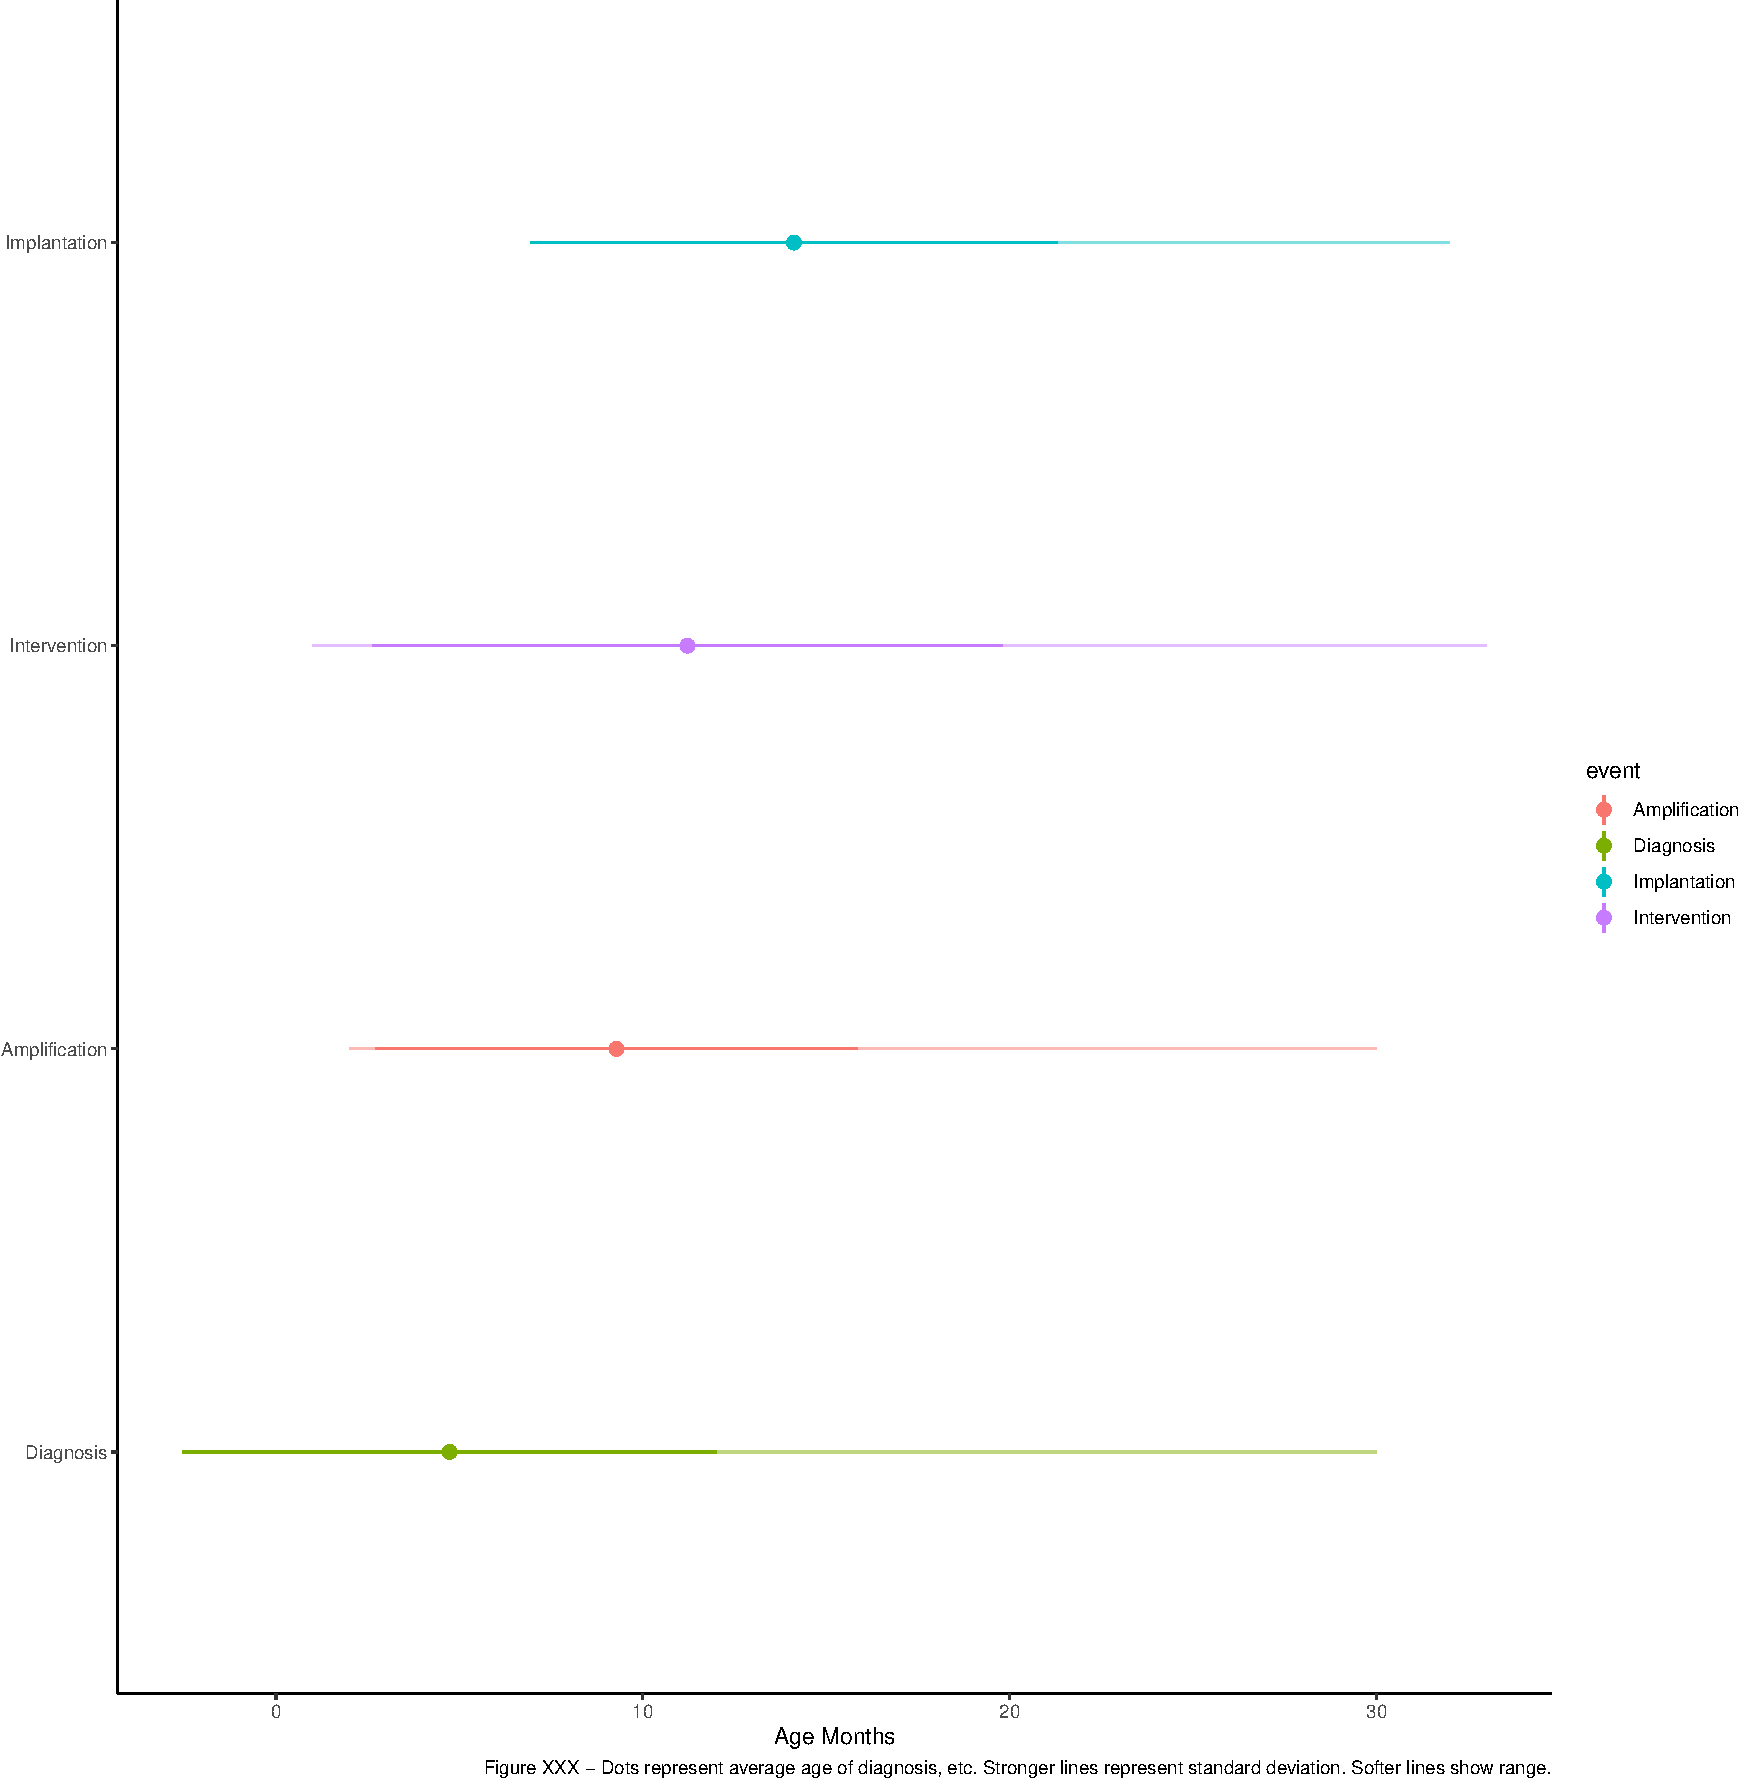
\includegraphics{ELSSP_paper_files/figure-latex/meets136-timeline-1.pdf}
\caption{\label{fig:meets136-timeline}Timeline for diagnosis/intervention/etc.}
\end{figure}

\begin{figure}
\centering
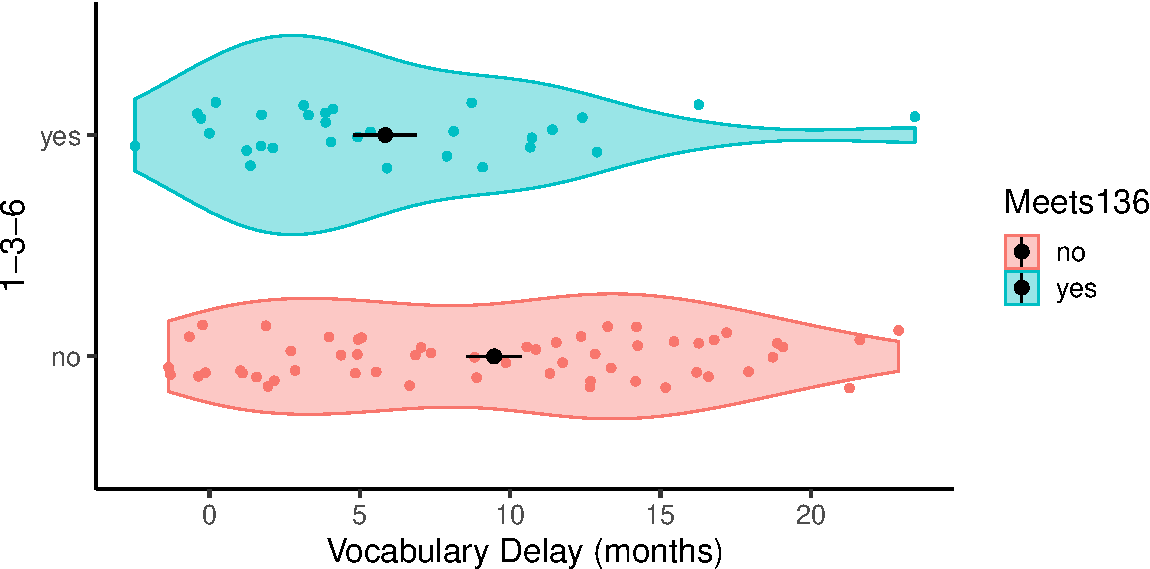
\includegraphics{ELSSP_paper_files/figure-latex/delay-violins-1.pdf}
\caption{\label{fig:delay-violins}Months delay for children who meet / don't meet 1-3-6 guidelines.}
\end{figure}

We first tested the link between 1-3-6 and vocabulary directly in an exploratory analysis. An independent samples t-test showed that children who did not meet 1-3-6 guidelines had significantly larger vocabulary delays than children who met 1-3-6 guidelines (\emph{t}(68.78)=2.62, \emph{p}=0.01; see Figure \ref{fig:delay-violins}). The group that did not meet 1-3-6 guidelines was 3.62 months more delayed with regard to vocabulary.

To better understand implementation of 1-3-6 guidelines, we next zoomed in on diagnosis and intervention. We conducted two linear regressions, one for age at diagnosis and one for age at intervention, considering only the predictors that would have been available or relevant at each of these stages (as detailed below). Model selection followed the same stepwise AIC-based process as Part II.

For age at diagnosis, we included the set of child-specific factors that would be relevant \emph{before} diagnosis of hearing loss (e.g., we excluded amplification type because a child would not receive a hearing aid or cochlear implant prior to being diagnosed with hearing loss.) We began with: gender, degree, developmental delay, health issues, prematurity, laterality, language background, and etiology.

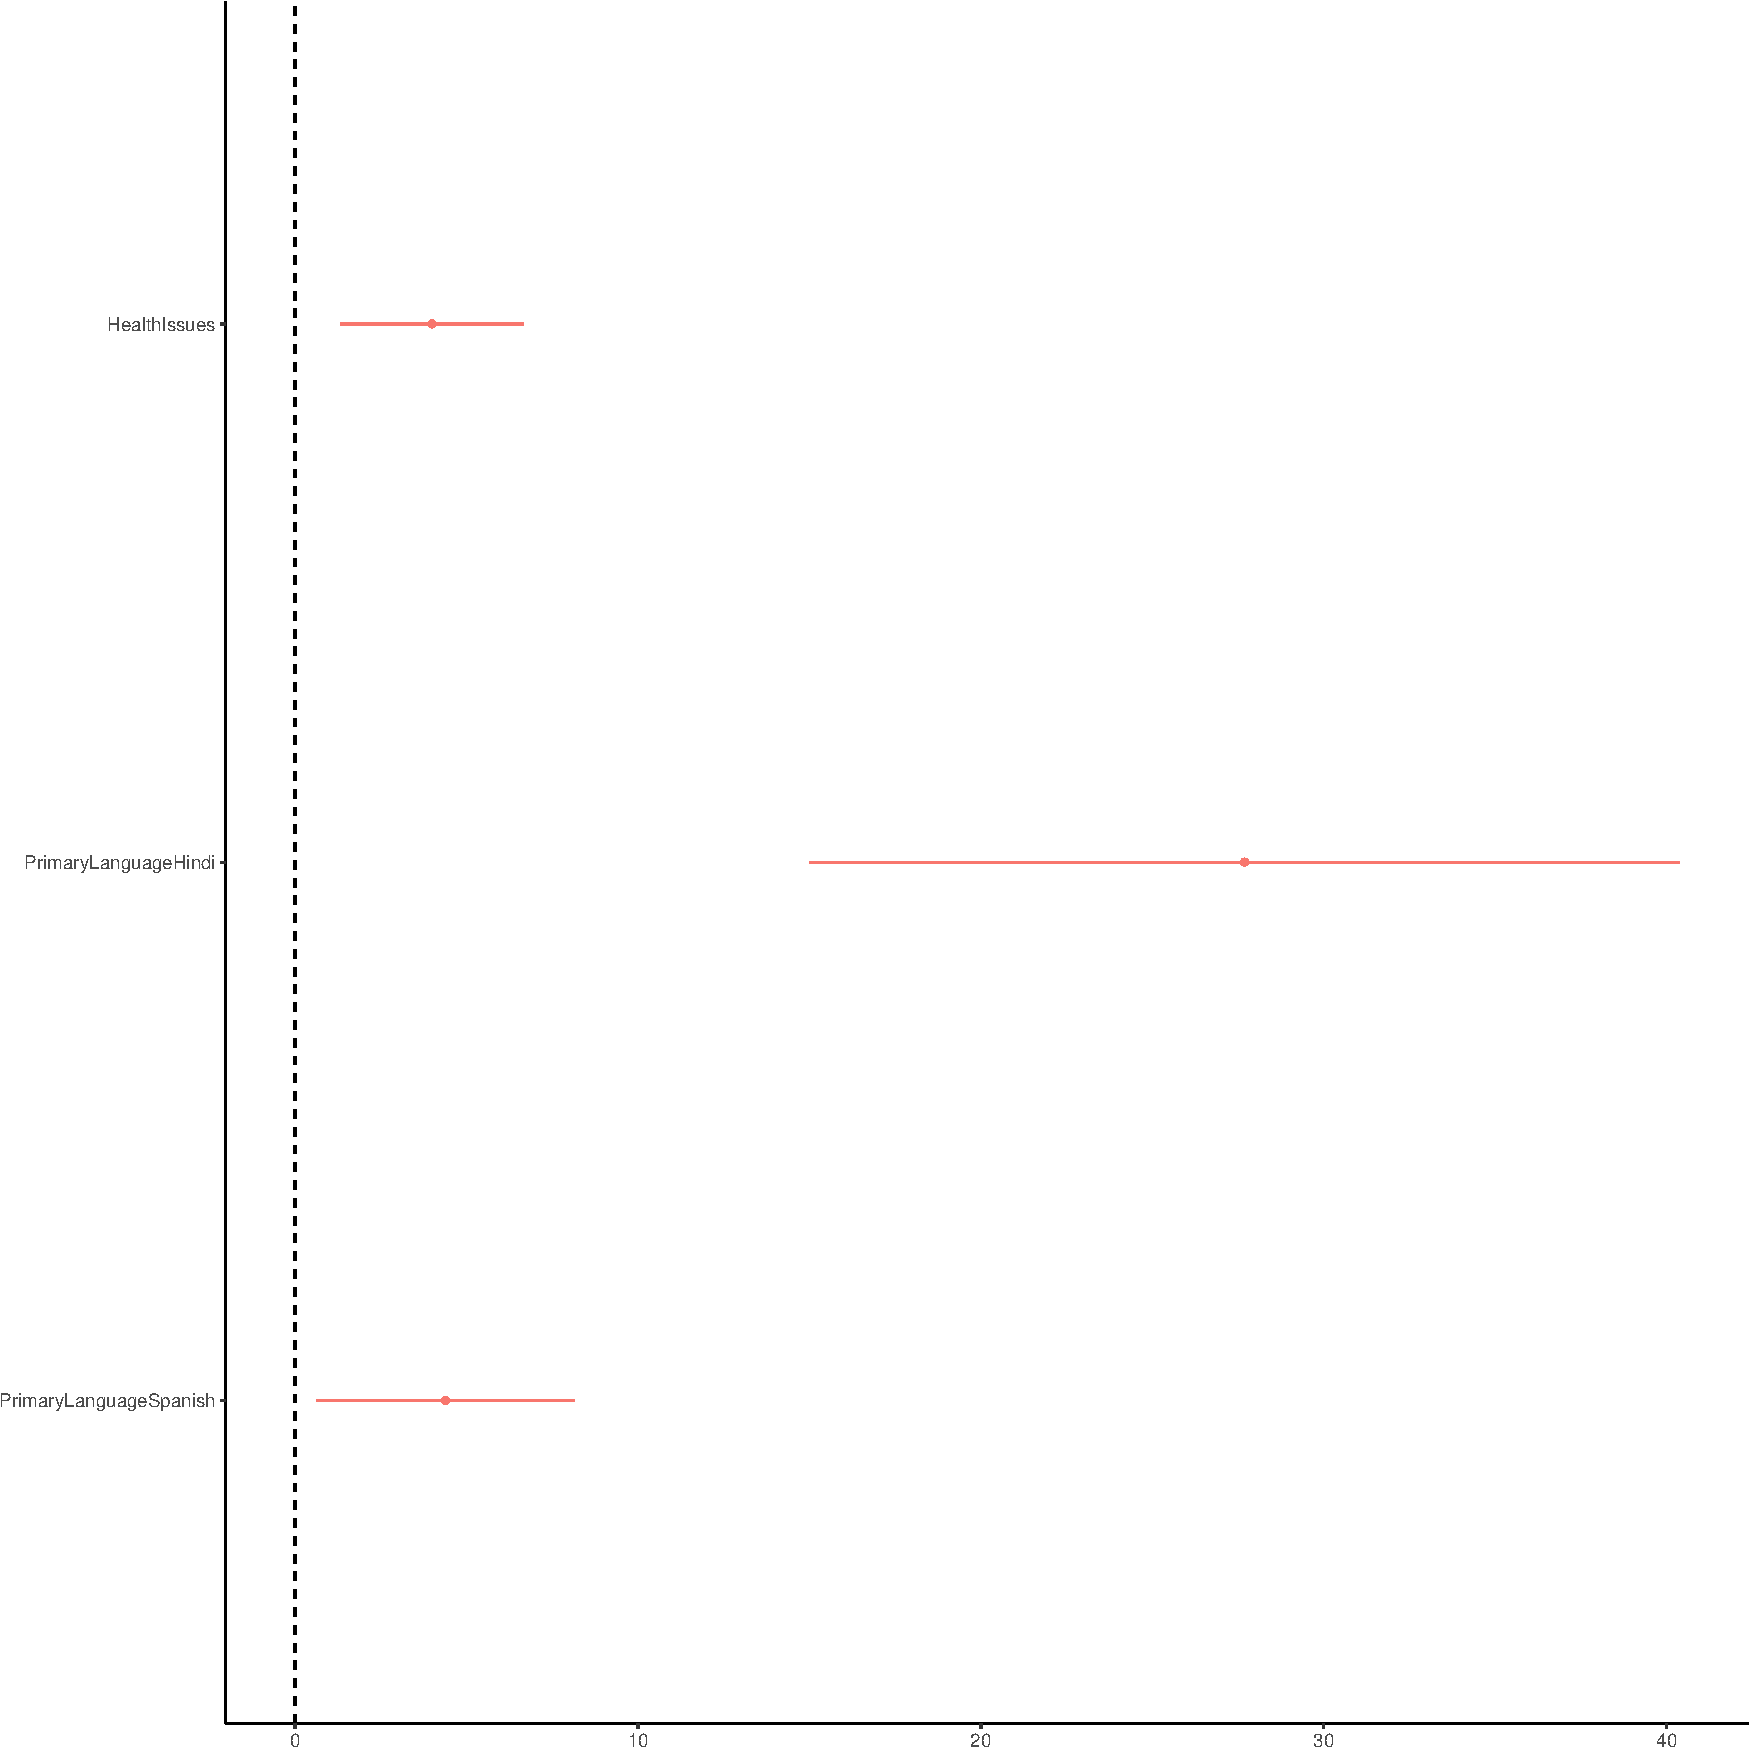
\includegraphics{ELSSP_paper_files/figure-latex/diagnosis-betas-1.pdf}

\begin{table}[H]
\centering
\begin{tabular}{l|r|r|r|r}
\hline
term & estimate & std.error & statistic & p.value\\
\hline
(Intercept) & 9.384015 & 1.967599 & 4.769272 & 0.0000069\\
\hline
HealthIssuesyes & 3.703441 & 1.418520 & 2.610778 & 0.0105472\\
\hline
Monolingual\_Englishyes & -6.469065 & 1.957318 & -3.305066 & 0.0013545\\
\hline
LateralityUnilateral & -2.148902 & 1.575573 & -1.363886 & 0.1759312\\
\hline
\end{tabular}
\end{table}

\begin{table}[H]
\centering
\begin{tabular}{l|r|r}
\hline
  & VIF & Df\\
\hline
HealthIssues & 1.002092 & 1\\
\hline
Monolingual\_English & 1.025896 & 1\\
\hline
Laterality & 1.027814 & 1\\
\hline
\end{tabular}
\end{table}

The best fit model was: Age at Diagnosis \textasciitilde{} Health Issues + Language Background + Laterality, with significant main effects of Health Issues and Language Background. This model accounted for 16.41\% of the variance in age at diagnosis (p = .001). Average age at dianosis was 4.65 months. Relative to English-speaking families, children from Spanish-speaking families were diagnosed 6.47 months later (p = .001). Children with health issues were diagnosed 3.70 months later than children without health issues (p = .01).

We repeated this model selection process for age at intervention. In addition to the variables used to fit the intervention model, we included age at diagnosis. The best fit model was: Age at Intervention \textasciitilde{} Premature Birth + Degree + Age at Diagnosis + Language Background (R\textsuperscript{2}=0.43 , p \textless{} .001; see Table ), with significant main effects of degree and age at diagnosis. Prematurity (ß = 3.78, p = .06) and language background (ß = -1.38, p = .52) were not significant predictors on their own, but their inclusion improved model fit. Average age at intervention was 11.12 months. More severe hearing loss predicted earlier intervention, such that for every additional 10 dB HL, predicted age at intervention was 4.02 weeks earlier (p \textless{} .01). With regard to age at diagnosis, for every month diagnosis was delayed, intervention was delayed by 2.84 weeks (p \textless{} .01).

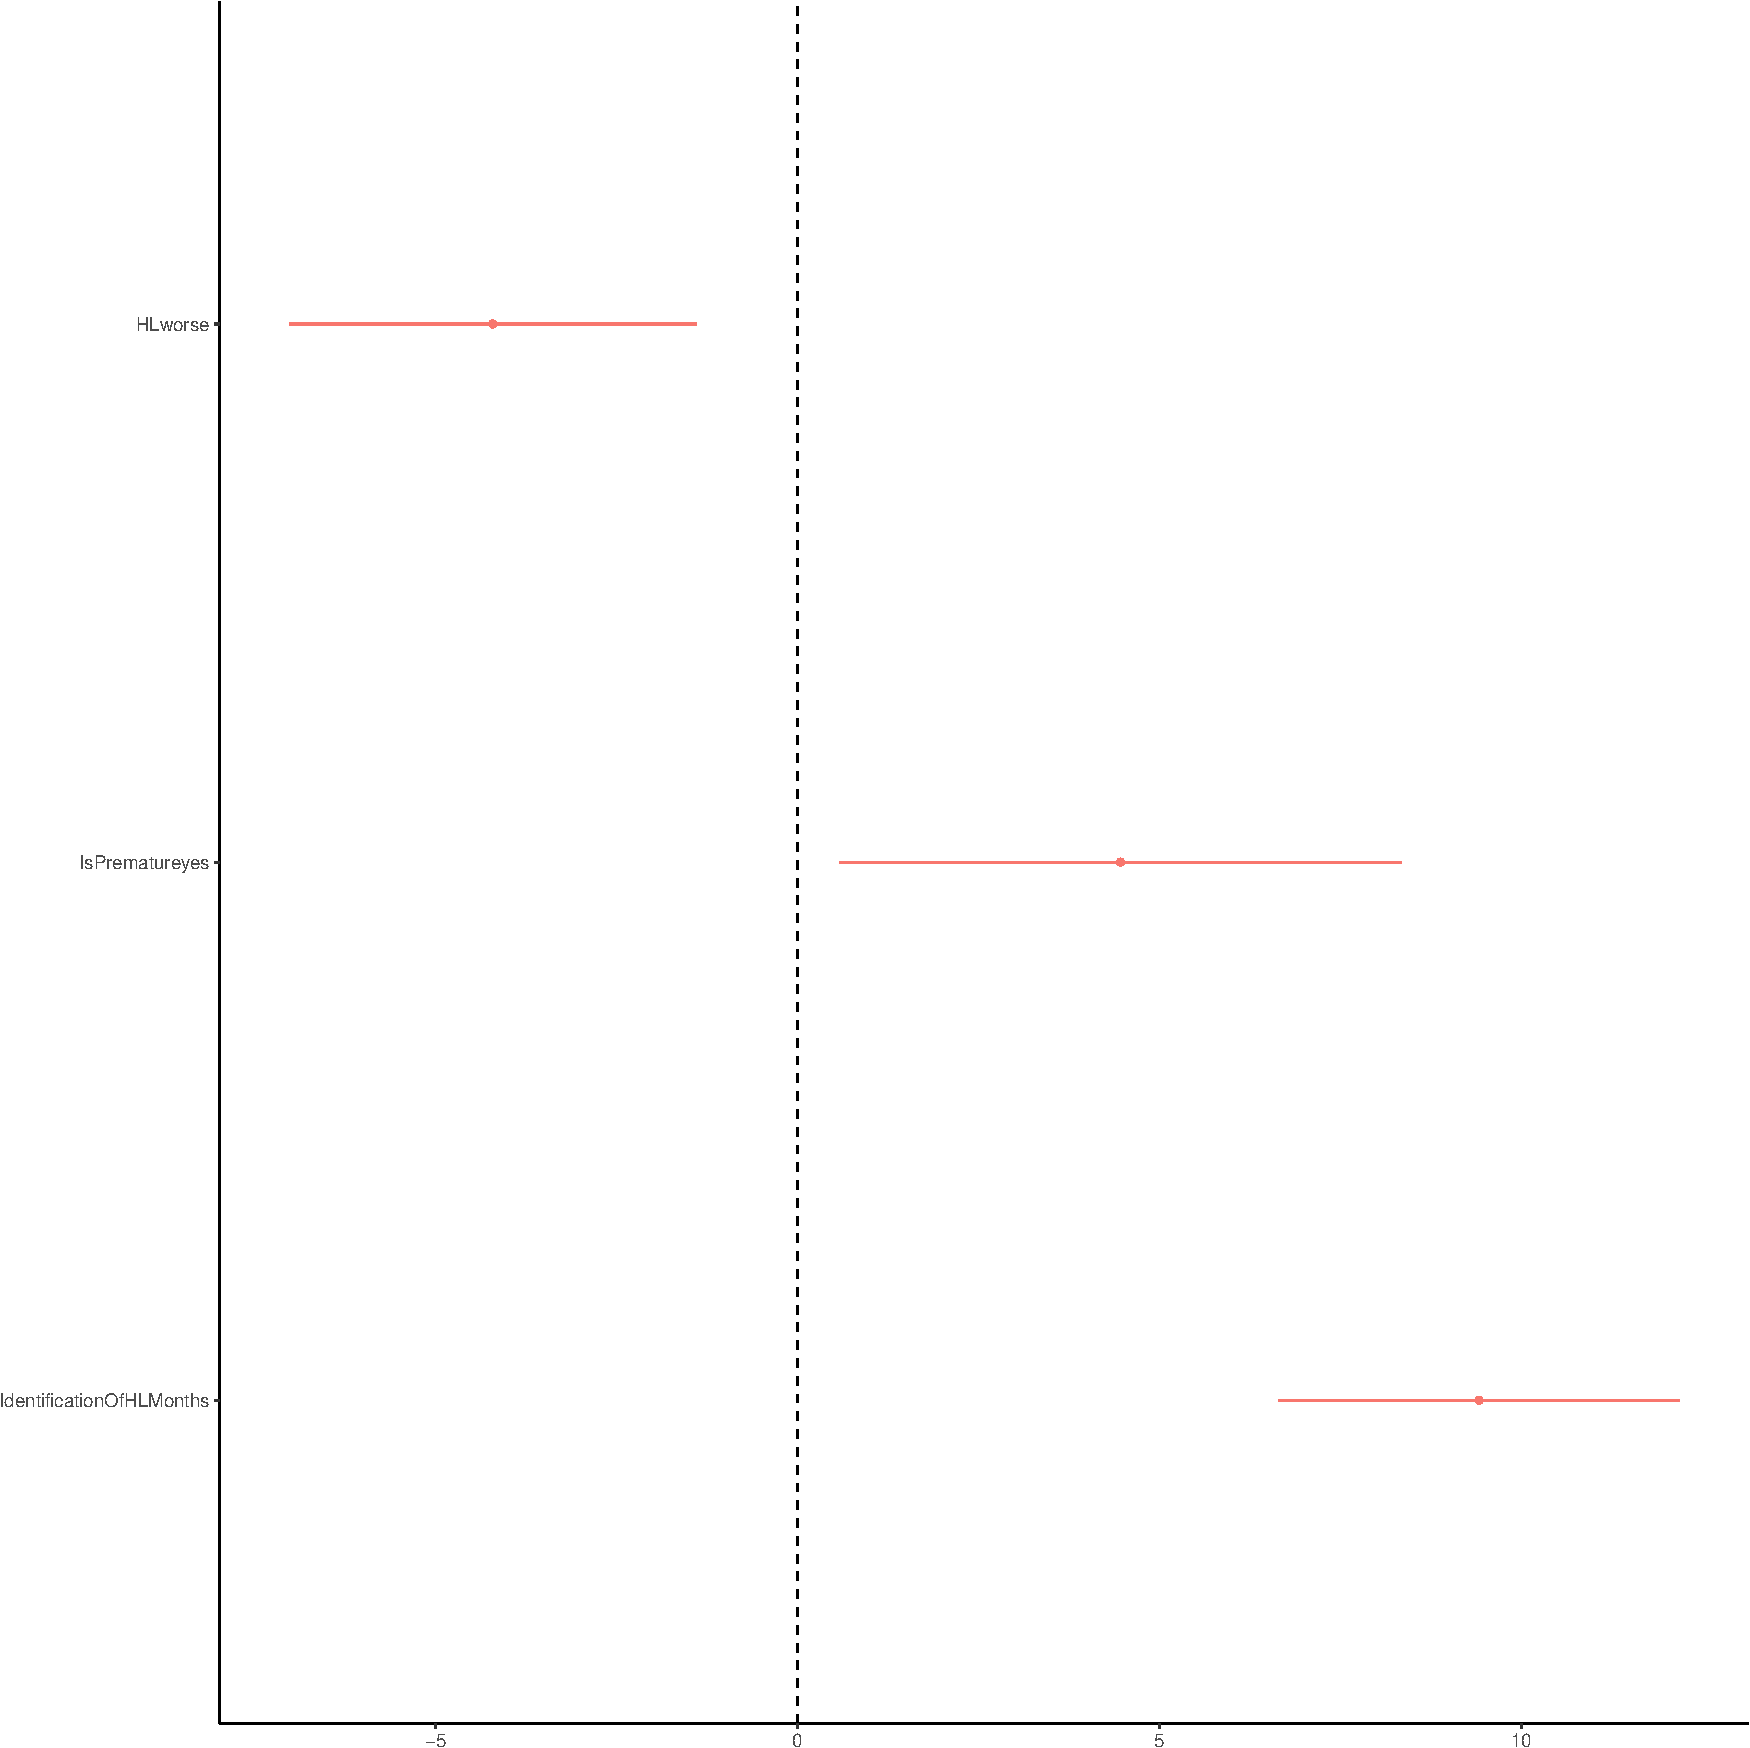
\includegraphics{ELSSP_paper_files/figure-latex/intervention-betas-1.pdf}

\begin{table}[H]
\centering
\begin{tabular}{l|r|r|r|r}
\hline
term & estimate & std.error & statistic & p.value\\
\hline
(Intercept) & 14.6545372 & 2.8717392 & 5.1030181 & 0.0000022\\
\hline
HLworse & -0.0925203 & 0.0302741 & -3.0560849 & 0.0030365\\
\hline
IsPrematureyes & 3.7839323 & 1.9540853 & 1.9364212 & 0.0563036\\
\hline
IdentificationOfHLMonths & 0.6520471 & 0.1044276 & 6.2440093 & 0.0000000\\
\hline
Monolingual\_Englishyes & -1.3846263 & 2.1177275 & -0.6538265 & 0.5150755\\
\hline
\end{tabular}
\end{table}

\begin{table}[H]
\centering
\begin{tabular}{l|r|r}
\hline
  & VIF & Df\\
\hline
HLworse & 1.030540 & 1\\
\hline
IsPremature & 1.064463 & 1\\
\hline
IdentificationOfHLMonths & 1.068221 & 1\\
\hline
Monolingual\_English & 1.101377 & 1\\
\hline
\end{tabular}
\end{table}

\hypertarget{discussion}{%
\section{Discussion}\label{discussion}}

In this study, we examined the demographic, audiological, and clinical characteristics of 100 young DHH children in North Carolina. We documented the distribution of these characteristics and explored the relationships between these variables, vocabulary, diagnosis, and intervention. In other, more-controlled samples, the variables studied here have been shown to be relevant for language development, but their effects are less well-understood \enquote{in the wild.} Here, we found complicated and nuanced relationships among the variables.

Returning to our original three questions, we asked first: how are child-level variables intertwined? We found significant non-random distribution of many of the variables, suggesting that in a real-world sample of children with hearing loss, many factors are not dissociable from each other. This was particularly true for many of the auditory characteristics and comorbid diagnoses; this paper provides the first population-based documentation of this distribution. We next asked whether these characteristics can predict vocabulary outcomes for DHH children. We created a model looking using all of our variables, but found that a model including only children's age, laterality of hearing loss, and amplification type best accounted for the variability in spoken vocabulary outcomes. Finally, we asked: how successful were the 1-3-6 guidelines for early detection and intervention, both in terms of improving child outcomes and ensuring timely diagnosis and intervention for all children with hearing loss? Here, we found that children who met 1-3-6 guidelines indeed had a smaller vocabulary delay. However, only 37\% of children met these guidelines. Some of the variability in when children received diagnosis / intervention could be explained by child characteristics.

Some readers might be left wondering what to take away from the complexity of these results, but the complexity itself is an important piece of understanding outcomes children with hearing loss. Taken together, these results demonstrate the connectedness of factors influencing outcomes for the diverse population of Deaf/Hard-of-Hearing children. We next highlight some possible implications of this study for future research and clinical practice.

\hypertarget{how-are-child-level-variables-intertwined}{%
\subsection{How are child-level variables intertwined?}\label{how-are-child-level-variables-intertwined}}

In our sample, we found significant overlap among demographic, audiological, and clinical variables. Prematurity, health issues, and developmental delay frequently co-occurred, such that children with one of these conditions were more likely to have any other condition. This is not surprising. Many conditions that cause developmental delays have a high incidence of health issues (e.g., heart problems in Down Syndrome; vomiting and seizures with hydrocephalus), and it is well documented that there is a higher incidence of developmental delay and health issues in preterm infants (Aarnoudse-Moens, Weisglas-Kuperus, van Goudoever, \& Oosterlaan, 2009; Costeloe et al., 2012; Luu, Katz, Leeson, Thébaud, \& Nuyt, 2016; Pierrat et al., 2017; Robertson et al., 2009; York \& DeVoe, 2002). In our sample, we also had a large range of health conditions (76 unique conditions in our sample of 100 children; see \ref{tab:comorbid-info} and Appendix XXX for more detailed information about comorbidities). Some studies to date have examined the outcomes of DHH children with certain conditions {[}e.g., XXX{]}. However, because the constellation of comorbid conditions is so varied, an important direction for future research could be whether cognitive and social abilities, as well as family's treatment resources, may be predictive of language outcomes across conditions.

We found that children with developmental delays (e.g., Down syndrome) were much more likely to use a total communication approach than typically-developing DHH children (i.e., total communication used by 59\% of DHH children with developmental delay vs.~10\% of typically-developing DHH children). Assignment to \enquote{spoken language} and \enquote{total communication} groups was not randomly distributed, with use of total communication appearing to follow children already at greater risk for verbal delays. Such a pattern is in line with clinical use of manual communication approaches for young children with disabilities (e.g., Branson \& Demchak, 2009). This should temper the interpretation of correlational studies finding links between total communication and language delays (e.g., Geers et al., 2017).

We also found relationships among many of our audiological variables. To highlight one such result, amplification devices were more common for children with less hearing (i.e., children with bilateral hearing loss and children with moderate to profound hearing loss). This may be due to the assumption that a hearing aid or cochlear implant will not benefit children with minimal hearing loss (Updike, 1994), although several studies have found benefits for amplification for mild or unilateral hearing loss (Briggs, Davidson, \& Lieu, 2011; Hassepass et al., 2013; Priwin, Jönsson, Hultcrantz, \& Granström, 2007; Walker et al., 2015; Winiger, Alexander, \& Diefendorf, 2016).

The relationships we documented in Part I are not necessarily surprising, given causal links among some of the variables (e.g., increased health issues in children born premature). Nevertheless, it should caution us to think critically about how we construct samples for controlled lab experiments. During study design: how likely is it to collect a desired sample of (e.g.) 32 typically-developing pediatric cochlear implant users with bilateral, severe-to-profound hearing loss, given that such a subsample may only represent roughly 14\% of the DHH population, as it does here? During interpretation of the results: how might the findings generalize to the rest of the DHH population given the constraints of the study at hand?

\hypertarget{predicting-vocabulary-outcomes}{%
\subsection{Predicting vocabulary outcomes}\label{predicting-vocabulary-outcomes}}

We next turn to how these variables may influence vocabulary outcomes. In our sample, 88.89\% of DHH children fell below the 50th percentile for spoken vocabulary/footnote\{Of the 11.11\% who were at or above the 50th percentile, 55.56\% were 8-to-9-month olds who were not yet producing any words (as expected at this age). \}. To have such a strong majority of DHH children below the 50th percentile for vocabulary development indicates that this group is not yet well-equipped to acquire spoken language. This disadvantage can have lasting consequences in the lives of DHH children (Karchmer \& Mitchell, 2003; Kyle \& Harris, 2010; Qi \& Mitchell, 2012).

In contrast to our predictions, the best model predicting vocabulary delay had just a few variables: age, amplification, and laterality. Notably, we did not simply find that DHH children were learning words at the same rate (albeit delayed) as hearing children, which would have led to a constant delay across developmental time. Instead, we see that the spoken vocabulary delay widens with age, indicating that the rate of spoken vocabulary acquisition is slower for DHH children. The result is a population increasingly behind on spoken language milestones, and given that none of the children here use sign language, on language development more broadly.

Few studies directly assess language development differences between unilateral and bilateral hearing loss. Our model results suggest that children with bilateral hearing loss are at a quantifiable disadvantage over children with unilateral hearing loss. However, children with unilateral hearing loss still experience notable delays both in the literature (Kiese-Himmel, 2002; Lieu, 2004, 2013; Lieu et al., 2012; Vila \& Lieu, 2015) and in our sample (Mean delay\_\{unilateral\} = 7.18). Similarly, in our sample, children without amplification were 3-4 months more delayed than children with hearing aids or cochlear implants. This increased delay for children without amplification or with bilateral hearing loss could reflect decreased spoken language audibility (Anne et al., 2017; Lieu, 2013; Tomblin et al., 2015; Vohr et al., 2008).

\hypertarget{predicting-early-diagnosis-and-intervention}{%
\subsection{Predicting early diagnosis and intervention}\label{predicting-early-diagnosis-and-intervention}}

Lastly, we explored the implementation of 1-3-6 guidelines. Only 36.84\% of children met the EHDI guidelines for diagnosis by 3 months and intervention by 6 months, despite ample evidence suggesting early diagnosis and intervention improve language outcomes (Apuzzo \& Yoshinaga-Itano, 1995; Ching et al., 2013; Holzinger et al., 2011; Kennedy et al., 2006; Robinshaw, 1995; Vohr et al., 2008, 2011; Watkin et al., 2007; White \& White, 1987; Yoshinaga-Itano et al., 1998, 2018). Children in our sample who met 1-3-6 guidelines were 3.62 months \emph{less} delayed in spoken vocabulary than children who were late to receive diagnosis and/or services. With these demonstrable benefits in mind, our sample, by dint of accepting all children receiving early intervention services in one state, was able to explore naturally occurring variance in who received on-time diagnosis and intervention.

\hypertarget{diagnosis}{%
\subsubsection{Diagnosis}\label{diagnosis}}

In the case of diagnosis, having health issues or a non-English language background predicted later diagnosis.
Children with health issues were diagnosed 3.70 months later than infants without health issues. One possible explanation is that the health issues caused acquired hearing loss that wouldn't be detected by the NBHS, thus delaying identification of hearing loss. In our sample, 16 of the 36 children with health issues had conditions that might cause acquired hearing loss (i.e., meningitis, sepsis, jaundice, seizures, hydrocephalus, MRSA, anemia, frequent fevers, cytomegalovirus). While acquired hearing loss may be one driver of delayed diagnosis for children with health issues, this accounts for only a fraction of the subpopulation with health issues. Another possible explanation is that the health issues required more pressing medical attention than the possible hearing loss. Families and medical providers had to prioritize treatment for the health issue (e.g., surgery for congenital heart defect) over diagnostic audiology services.

Infants from Spanish-speaking families were diagnosed 3.78 months later than infants from English-speaking families. This may be due to cultural differences in attitudes towards deafness (Caballero, Muñoz, Schultz, Graham, \& Meibos, 2018; Rodriguez \& Allen, 2020; Steinberg, Dávila, Collazo, Loew, \& Fischgrund, 1997, @steinberg2003) or it may result from a lack of linguistically accessible and culturally appropriate audiology services. Only 5.6\% of American audiologists identify as a bilingual service provider (ASHA, 2019), and services from a monolingual provider may be insufficient. To this point, Caballero et al. (2017) found that Hispanic-American parents of DHH children wish for more concrete resources, comprehensive information, and emotional support from their audiologist. In a nationwide survey of audiologists, the majority of audiologists reported that language barriers presented a major challenge in working with Spanish-speaking families, specifically in obtaining the child's case history and providing recommendations for follow-up services (Abreu, Adriatico, \& DePierro, 2011).

\hypertarget{intervention}{%
\subsubsection{Intervention}\label{intervention}}

As expected, more severe hearing loss predicted earlier intervention, such that for every additional 10 dB HL, predicted age at intervention was 4.02 weeks earlier. This converges with findings by Harrison, Roush, and Wallace (2003) in which severe-to-profound hearing loss was diagnosed 2-5 months earlier than mild-to-moderate hearing loss. Parents and clinicians may adopt a wait-and-see approach to intervention for children with some residual hearing. Nevertheless, mild-to-moderate hearing loss is associated with language delays and academic challenges (Blair et al., 1985; Delage \& Tuller, 2007), which early intervention may offset.

Age at start of services was also associated with age at diagnosis: for every month diagnosis was delayed, intervention was delayed by 2.84 weeks. Early diagnosis puts children in the pipeline towards intervention earlier. Ching et al. (2013) found that age at intervention predicted better outcomes for DHH children, above and beyond age at diagnosis. Of course, these two variables are related, such that we cannot hope to achieve early intervention goals without ensuring children receive timely diagnosis.

A final point regarding 1-3-6 attainment: this sample is composed of children receiving birth-to-3 services. An estimated 67\% of children with hearing loss enroll in early intervention services (CDC, 2018). While this represents a tremendous step forward in prompt early intervention services relative to just a few decades prior, early intervention may not be early enough. Less than 39\% of our sample of children in early intervention meet the 6-month EHDI benchmark. Furthermore, an unknown fraction of the DHH population in North Carolina aren't included in this analysis because they have not been enrolled in services by 36 months. The AAP estimates that almost 36\% of infants who do not pass a newborn hearing screening are lost to follow-up. Assuming that the population of children in early intervention only represents two thirds of the population with hearing loss, our data suggest that the actual proportion of DHH children who receive intervention by the EHDI-recommended 6 months may be closer to 26\%. These children may not receive clinical support until school-age or later.

\hypertarget{educational-and-clinical-implications}{%
\subsection{Educational and Clinical Implications}\label{educational-and-clinical-implications}}

Despite high rates of NBHS in North Carolina, and even relatively high rates of diagnosis by 3 months (66/100 children in our sample), most children in our sample did not meet the 1-3-6 guidelines. Based on our analyses, we have the following recommendations for increasing attainment of 1-3-6 guidelines:

\begin{enumerate}

\item Frequent hearing screenings for children receiving medical or therapeutic care for health issues.
\item Service coordination for families balancing multiple co-occurring conditions.
\item Expansion of bilingual clinicians both in-person and teletherapy clinicians to provide therapy and service coordination to non-English-speaking families.
\item Provision and encouragement of early intervention services for children with mild to moderate hearing loss.

\end{enumerate}

Additionally, the vast majority of children in our sample experienced vocabulary delays (relative to hearing peers), and studies of spoken vocabulary development in older DHH children suggest that they may not catch up (Lund, 2016). This should set clinicians and educators on high alert, due to the demonstrated importance of vocabulary skills in literacy (Biemiller, 2003; Hemphill \& Tivnan, 2008; Stæhr, 2008) and in education more broadly (e.g., Young, 2005; Monroe \& Orme, 2002). As early intervention predicts vocabulary outcomes in study after study (including this present study and e.g., Vohr et al., 2008, 2011; Ching et al., 2018, 2013; Holzinger et al., 2011; Watkin et al., 2007), ensuring intervention by 6 months for all DHH children may be one way to address spoken vocabulary deficits. Another solution: even prior to intervention or amplification, provision of structured, accessible language input (i.e., sign language) may mitigate negative effects of auditory deprivation on language skills (Davidson, Lillo-Martin, \& Pichler, 2014; Hassanzadeh, 2012; Spellun \& Kushalnagar, 2018). Indeed, while we recognize that learning sign language may pose a challenge for some families for myriad reasons, and as noted above, our sample did not use sign language, we nevertheless feel it is worth underscoring as an important language support for DHH children and their families.

In recommending sign language, we follow the rationale set forth by Hall, Hall, and Caselli (2019), summarized here: Spoken language outcomes for DHH children are variable and unpredictable (Ganek, McConkey Robbins, \& Niparko, 2012; Szagun \& Schramm, 2016), and even in optimal situations, many DHH children do not achieve age-appropriate spoken language outcomes (e.g., Geers et al., 2017). Failing to achieve language proficiency (in any language) confers higher risk of disrupted cognitive, academic, and socioemotional development (Amraei, Amirsalari, \& Ajalloueyan, 2017; Dammeyer, 2010; Desselle, 1994; Hall et al., 2017; Hrastinski \& Wilbur, 2016; Kushalnagar et al., 2011; Moeller \& Schick, n.d.; Preisler, Tvingstedt, \& Ahlström, 2002; Schick, De Villiers, De Villiers, \& Hoffmeister, 2007). The available data do not suggest that sign language harms spoken language development (Davidson et al., 2014; Park et al., 2013), and in fact, some studies suggest that sign language \emph{benefits} spoken language development (e.g., Hassanzadeh, 2012). Providing early access to a natural sign language offers children another path to language mastery, and use of sign language does not preclude learning spoken language. Thus, we encourage sign language use \emph{at least} prior to mastery of spoken language, and when possible for the family, we encourage its continued use as a language resource.

\hypertarget{limitations-and-opportunities-for-future-work}{%
\section{Limitations and Opportunities for Future Work}\label{limitations-and-opportunities-for-future-work}}

This study represents an important first step in quantifying variability in demographic characteristics, language outcomes, and 1-3-6 attainment. However, due to the exploratory nature of the study, its limited geographic scope, and the variability of the same, it may be unclear what readers should take away from these results. These potential limitations represent opportunities for future investigators to better understand the complex factors influencing DHH children's outcomes.

These analyses were exploratory, and there were many possible analytic routes. That said, our results largely converge with or replicate key aspects of past studies (e.g., Ching et al., 2013) and received wisdom among clinicians. In the interest of transparency, these data and all code generating our results are available on our OSF page (XXX) and we encourage those interested to explore further analyses.

This sample is composed only of children in North Carolina, and certain factors vary by country and by state (e.g., diagnosis and early intervention practices; NAD, n.d.). However, based on other demographic research (Blackorby \& Knokey, 2006; Institute, 2014), our sample largely resembles the national DHH population in terms of degree of hearing loss, percentage of children with additional disabilities, cochlear implant and hearing aid use, language background, and gender. We would exercise caution in applying these results to regions where sign language access for DHH children is more common (e.g.~Washington D.C.; Rochester, New York.) A similar naturalistic study in those regions could help illuminate the effects of different clinical and demographic factors in a signing population

Furthermore, the considerable variability in the sample did not allow us to easily isolate effects of different characteristics. However, this variability is real-world variability, and as we demonstrated earlier, many of these variables co-occurred such that it may not make sense to isolate. Larger sample sizes, which are often difficult to achieve in research with DHH children, would help to tease apart different effects. As researchers continue to study influences on vocabulary in DHH children, a meta-analytic approach may be able to better estimate effects and effect sizes within the varied outcomes of this diverse population.

\hypertarget{conclusion}{%
\section{Conclusion}\label{conclusion}}

Using a diverse sample of 100 children enrolled in early intervention, we provide a description of children's demographic and audiological characteristics, vocabulary outcomes, and clinical milestones. Our results suggest that the children's characteristics of young DHH children have implications for other characteristics, vocabulary outcomes, and timing of clinical intervention.

\pagebreak

\hypertarget{references}{%
\section*{References}\label{references}}
\addcontentsline{toc}{section}{References}

\hypertarget{refs}{}
\leavevmode\hypertarget{ref-2000}{}%
15A NCAC 21F .1201 - .1204. (2000).

\leavevmode\hypertarget{ref-aarnoudse-moens2009}{}%
Aarnoudse-Moens, C. S. H., Weisglas-Kuperus, N., van Goudoever, J. B., \& Oosterlaan, J. (2009). Meta-analysis of neurobehavioral outcomes in very preterm and/or very low birth weight children. \emph{Pediatrics}, \emph{124}(2), 717--728. \url{https://doi.org/10.1542/peds.2008-2816}

\leavevmode\hypertarget{ref-abreu2011}{}%
Abreu, R. A., Adriatico, T., \& DePierro, A. (2011). QUÉ PASA?: ``What's Happening'' in Overcoming Barriers to Serving Bilingual Children? \emph{The ASHA Leader}, \emph{16}(13). \url{https://doi.org/10.1044/leader.FTR2.16132011.12}

\leavevmode\hypertarget{ref-amin2014}{}%
Amin, S. B., Vogler-Elias, D., Orlando, M., \& Wang, H. (2014). Auditory neural myelination is associated with early childhood language development in premature infants. \emph{Early Human Development}, \emph{90}(10), 673--678. \url{https://doi.org/10.1016/j.earlhumdev.2014.07.014}

\leavevmode\hypertarget{ref-amraei2017}{}%
Amraei, K., Amirsalari, S., \& Ajalloueyan, M. (2017). Comparison of intelligence quotients of first- and second-generation deaf children with cochlear implants. \emph{International Journal of Pediatric Otorhinolaryngology}, \emph{92}, 167--170. \url{https://doi.org/10.1016/j.ijporl.2016.10.005}

\leavevmode\hypertarget{ref-anderson2002}{}%
Anderson, D., \& Reilly, J. (2002). The MacArthur Communicative Development Inventory: Normative Data for American Sign Language. \emph{Journal of Deaf Studies and Deaf Education}, \emph{7}(2), 83--106. \url{https://doi.org/10.1093/deafed/7.2.83}

\leavevmode\hypertarget{ref-anne2017}{}%
Anne, S., Lieu, J. E. C., \& Cohen, M. S. (2017). Speech and Language Consequences of Unilateral Hearing Loss: A Systematic Review. \emph{Otolaryngologyhead and Neck Surgery : Official Journal of American Academy of Otolaryngology-Head and Neck Surgery}, \emph{157}(4), 572--579. \url{https://doi.org/10.1177/0194599817726326}

\leavevmode\hypertarget{ref-apuzzo1995}{}%
Apuzzo, M.-R. L., \& Yoshinaga-Itano, C. (1995). \emph{Early Identification of Infants with Significant Hearing Loss and the Minnesota Child Development Inventory} (No. 2). \emph{SEMINARS IN HEARING-VOLUME} (Vol. 16).

\leavevmode\hypertarget{ref-artieres2009}{}%
Artières, F., Vieu, A., Mondain, M., Uziel, A., \& Venail, F. (2009). Impact of early cochlear implantation on the linguistic development of the deaf child. \emph{Otology and Neurotology}, \emph{30}(6), 736--742. \url{https://doi.org/10.1097/MAO.0b013e3181b2367b}

\leavevmode\hypertarget{ref-asha2019}{}%
ASHA. (2019). Demographic Profile of ASHA Members Providing Bilingual Services, Year-End 2019, 6.

\leavevmode\hypertarget{ref-barre2011}{}%
Barre, N., Morgan, A., Doyle, L. W., \& Anderson, P. J. (2011). Language abilities in children who were very preterm and/or very low birth weight: A meta-analysis. \emph{Journal of Pediatrics}, \emph{158}(5). \url{https://doi.org/10.1016/j.jpeds.2010.10.032}

\leavevmode\hypertarget{ref-biemiller2003}{}%
Biemiller, A. (2003). Vocabulary: Needed If More Children Are to Read Well. \emph{Reading Psychology}, \emph{24}(3-4), 323--335. \url{https://doi.org/10.1080/02702710390227297}

\leavevmode\hypertarget{ref-birman2012}{}%
Birman, C. S., Elliott, E. J., \& Gibson, W. P. (2012). Pediatric cochlear implants: Additional disabilities prevalence, risk factors, and effect on language outcomes. \emph{Otology and Neurotology}, \emph{33}(8), 1347--1352. \url{https://doi.org/10.1097/MAO.0b013e31826939cc}

\leavevmode\hypertarget{ref-blackorby2006}{}%
Blackorby, J., \& Knokey, A.-M. (2006). A National Profile of Students with Hearing Impairments in Elementary and Middle School: A Special Topic Report from the Special Education Elementary Longitudinal Study, 30.

\leavevmode\hypertarget{ref-blair1985}{}%
Blair, J. C., Peterson, M., \& Viehweg, S. (1985). The Effects of Mild Sensorineural Hearing Loss on Academic Performance of Young School-Age Children. \emph{Volta Review}, \emph{87}(2), 87--93.

\leavevmode\hypertarget{ref-bornstein2004}{}%
Bornstein, M. H., Hahn, C.-S., \& Haynes, O. M. (2004). Specific and general language performance across early childhood: Stability and gender considerations. \emph{First Language}, \emph{24}(3), 267--304. \url{https://doi.org/10.1177/0142723704045681}

\leavevmode\hypertarget{ref-branson2009}{}%
Branson, D., \& Demchak, M. (2009). The Use of Augmentative and Alternative Communication Methods with Infants and Toddlers with Disabilities: A Research Review. \emph{Augmentative and Alternative Communication}, \emph{25}(4), 274--286. \url{https://doi.org/10.3109/07434610903384529}

\leavevmode\hypertarget{ref-briggs2011}{}%
Briggs, L., Davidson, L., \& Lieu, J. E. C. (2011). Outcomes of conventional amplification for pediatric unilateral hearing loss. \emph{The Annals of Otology, Rhinology, and Laryngology}, \emph{120}(7), 448--454. \url{https://doi.org/10.1177/000348941112000705}

\leavevmode\hypertarget{ref-bruce2015}{}%
Bruce, S. M., \& Borders, C. (2015). Communication and Language in Learners Who Are Deaf and Hard of Hearing With Disabilities: Theories, Research, and Practice. \emph{American Annals of the Deaf}, \emph{160}(4), 368--384. \url{https://doi.org/10.1353/aad.2015.0035}

\leavevmode\hypertarget{ref-caballero2018}{}%
Caballero, A., Muñoz, K., Schultz, J., Graham, L., \& Meibos, A. (2018). Hispanic Parents' Beliefs, Attitudes and Perceptions Toward Pediatric Hearing Loss: A Comprehensive Literature Review. In. \url{https://doi.org/10.26077/h0tf-ve32}

\leavevmode\hypertarget{ref-caballero2017}{}%
Caballero, A., Muñoz, K., White, K., Nelson, L., Domenech-Rodriguez, M., \& Twohig, M. (2017). Pediatric Hearing Aid Management: Challenges among Hispanic Families. \emph{Journal of the American Academy of Audiology}, \emph{28}(8), 718--730. \url{https://doi.org/10.3766/jaaa.16079}

\leavevmode\hypertarget{ref-capps2009}{}%
Capps, L. (2009). H.R.1246 - 111th Congress (2009-2010): Early Hearing Detection and Intervention Act of 2009.

\leavevmode\hypertarget{ref-carter2017}{}%
Carter, F. A., \& Msall, M. E. (2017). \emph{Language Abilities as a Framework for Understanding Emerging Cognition and Social Competencies after Late, Moderate, and Very Preterm Birth}. \emph{Journal of Pediatrics} (Vol. 181). Mosby Inc. \url{https://doi.org/10.1016/j.jpeds.2016.10.077}

\leavevmode\hypertarget{ref-castellanos2016}{}%
Castellanos, I., Pisoni, D. B., Kronenberger, W. G., \& Beer, J. (2016). Early expressive language skills predict long-term neurocognitive outcomes in cochlear implant users: Evidence from the MacArthurBates Communicative Development Inventories. \emph{American Journal of Speech-Language Pathology}, \emph{25}(3), 381--392. \url{https://doi.org/10.1044/2016_AJSLP-15-0023}

\leavevmode\hypertarget{ref-cdc2018}{}%
CDC. (2018). 2016 Hearing Screening Summary. \emph{Centers for Disease Control and Prevention}. https://www.cdc.gov/ncbddd/hearingloss/2016-data/01-data-summary.html.

\leavevmode\hypertarget{ref-chapman1997}{}%
Chapman, R. S. (1997). Language development in children and adolescents with Down syndrome. \emph{Mental Retardation and Developmental Disabilities Research Reviews}, \emph{3}(4), 307--312. \href{https://doi.org/10.1002/(SICI)1098-2779(1997)3:4\%3C307::AID-MRDD5\%3E3.0.CO;2-K}{https://doi.org/10.1002/(SICI)1098-2779(1997)3:4\textless{}307::AID-MRDD5\textgreater{}3.0.CO;2-K}

\leavevmode\hypertarget{ref-ching2018}{}%
Ching, T. Y. C., Dillon, H., Leigh, G., \& Cupples, L. (2018). Learning from the Longitudinal Outcomes of Children with Hearing Impairment (LOCHI) study: Summary of 5-year findings and implications. \emph{International Journal of Audiology}, \emph{57}(sup2), S105--S111. \url{https://doi.org/10.1080/14992027.2017.1385865}

\leavevmode\hypertarget{ref-ching2010}{}%
Ching, T. Y., Crowe, K., Martin, V., Day, J., Mahler, N., Youn, S., \ldots{} Orsini, J. (2010). Language development and everyday functioning of children with hearing loss assessed at 3 years of age. In \emph{International Journal of Speech-Language Pathology} (Vol. 12, pp. 124--131). \url{https://doi.org/10.3109/17549500903577022}

\leavevmode\hypertarget{ref-ching2013}{}%
Ching, T. Y., Dillon, H., Marnane, V., Hou, S., Day, J., Seeto, M., \ldots{} Yeh, A. (2013). Outcomes of early- and late-identified children at 3 years of age: Findings from a prospective population-based study. \emph{Ear and Hearing}, \emph{34}(5), 535--552. \url{https://doi.org/10.1097/AUD.0b013e3182857718}

\leavevmode\hypertarget{ref-ching2007}{}%
Ching, T. Y., Van Wanrooy, E., \& Dillon, H. (2007). \emph{Binaural-Bimodal Fitting or Bilateral Implantation for Managing Severe to Profound Deafness: A Review}. \emph{Trends in Amplification} (Vol. 11). \url{https://doi.org/10.1177/1084713807304357}

\leavevmode\hypertarget{ref-clark1981}{}%
Clark, J. G. (1981). Uses and abuses of hearing loss classification. \emph{ASHA: A Journal of the American Speech-Language-Hearing Association}, \emph{23}(7), 493--500.

\leavevmode\hypertarget{ref-clark2016}{}%
Clark, M. D., Hauser, P. C., Miller, P., Kargin, T., Rathmann, C., Guldenoglu, B., \ldots{} Israel, E. (2016). The Importance of Early Sign Language Acquisition for Deaf Readers. \emph{Reading and Writing Quarterly}, \emph{32}(2), 127--151. \url{https://doi.org/10.1080/10573569.2013.878123}

\leavevmode\hypertarget{ref-costeloe2012}{}%
Costeloe, K. L., Hennessy, E. M., Haider, S., Stacey, F., Marlow, N., \& Draper, E. S. (2012). Short term outcomes after extreme preterm birth in England: Comparison of two birth cohorts in 1995 and 2006 (the EPICure studies). \emph{BMJ (Clinical Research Ed.)}, \emph{345}, e7976. \url{https://doi.org/10.1136/bmj.e7976}

\leavevmode\hypertarget{ref-cupples2014}{}%
Cupples, L., Ching, T. Y. C., Crowe, K., Seeto, M., Leigh, G., Street, L., \ldots{} Thomson, J. (2014). Outcomes of 3-year-old children with hearing loss and different types of additional disabilities. \emph{Journal of Deaf Studies and Deaf Education}, \emph{19}(1), 20--39. \url{https://doi.org/10.1093/deafed/ent039}

\leavevmode\hypertarget{ref-cupples2018}{}%
Cupples, L., Ching, T. Y. C., Leigh, G., Martin, L., Gunnourie, M., Button, L., \ldots{} Van Buynder, P. (2018). Language development in deaf or hard-of-hearing children with additional disabilities: Type matters! \emph{Journal of Intellectual Disability Research: JIDR}, \emph{62}(6), 532--543. \url{https://doi.org/10.1111/jir.12493}

\leavevmode\hypertarget{ref-cusson2003}{}%
Cusson, R. M. (2003). Factors influencing language development in preterm infants. \emph{Journal of Obstetric, Gynecologic, and Neonatal Nursing : JOGNN / NAACOG}, \emph{32}(3), 402--409. \url{https://doi.org/10.1177/0884217503253530}

\leavevmode\hypertarget{ref-dammeyer2010}{}%
Dammeyer, J. (2010). Psychosocial Development in a Danish Population of Children With Cochlear Implants and Deaf and Hard-of-Hearing Children. \emph{The Journal of Deaf Studies and Deaf Education}, \emph{15}(1), 50--58. \url{https://doi.org/10.1093/deafed/enp024}

\leavevmode\hypertarget{ref-davidson2014}{}%
Davidson, K., Lillo-Martin, D., \& Pichler, D. C. (2014). Spoken english language development among native signing children with cochlear implants. \emph{Journal of Deaf Studies and Deaf Education}, \emph{19}(2), 239--250. \url{https://doi.org/10.1093/deafed/ent045}

\leavevmode\hypertarget{ref-dediego-lazaro2018}{}%
de Diego-Lázaro, B., Restrepo, M. A., Sedey, A. L., \& Yoshinaga-Itano, C. (2018). Predictors of Vocabulary Outcomes in Children Who Are Deaf or Hard of Hearing From Spanish-Speaking Families. \emph{Language, Speech, and Hearing Services in Schools}, \emph{50}(1), 1--13. \url{https://doi.org/10.1044/2018_LSHSS-17-0148}

\leavevmode\hypertarget{ref-delage2007}{}%
Delage, H., \& Tuller, L. (2007). Language development and mild-to-moderate hearing loss: Does language normalize with age? \emph{Journal of Speech, Language, and Hearing Research}, \emph{50}(5), 1300--1313. \url{https://doi.org/10.1044/1092-4388(2007/091)}

\leavevmode\hypertarget{ref-desselle1994}{}%
Desselle, D. D. (1994). Self-esteem, family climate, and communication patterns in relation to deafness. \emph{American Annals of the Deaf}, \emph{139}(3), 322--328. \url{https://doi.org/10.1353/aad.2012.0295}

\leavevmode\hypertarget{ref-dettman2007}{}%
Dettman, S. J., Pinder, D., Briggs, R. J., Dowell, R. C., \& Leigh, J. R. (2007). Communication development in children who receive the cochlear implant younger than 12 months: Risks versus benefits. \emph{Ear and Hearing}, \emph{28}(SUPPL.2). \url{https://doi.org/10.1097/AUD.0b013e31803153f8}

\leavevmode\hypertarget{ref-dillon2004}{}%
Dillon, C. M., Burkholder, R. A., Cleary, M., \& Pisoni, D. B. (2004). Nonword repetition by children with cochlear implants: Accuracy ratings from normal-hearing listeners. \emph{Journal of Speech, Language, and Hearing Research}, \emph{47}(5), 1103--1116. \url{https://doi.org/10.1044/1092-4388(2004/082)}

\leavevmode\hypertarget{ref-ehdi}{}%
EHDI. (n.d.). Early Hearing Detection and Intervention (EHDI). \emph{AAP.org}. http://www.aap.org/en-us/advocacy-and-policy/aap-health-initiatives/PEHDIC/Pages/Early-Hearing-Detection-and-Intervention.aspx.

\leavevmode\hypertarget{ref-eisenberg2007}{}%
Eisenberg, L. S. (2007). Current state of knowledge: Speech recognition and production in children with hearing impairment. \emph{Ear and Hearing}, \emph{28}(6), 766--772. \url{https://doi.org/10.1097/AUD.0b013e318157f01f}

\leavevmode\hypertarget{ref-fenson1994}{}%
Fenson, L., Dale, P. S., Reznick, J. S., Bates, E., Thal, D. J., Pethick, S. J., \ldots{} Stiles, J. (1994). Variability in Early Communicative Development. \emph{Monographs of the Society for Research in Child Development}, \emph{59}(5), i. \url{https://doi.org/10.2307/1166093}

\leavevmode\hypertarget{ref-frank2019}{}%
Frank, M., Braginsky, M., Marchman, V., \& Yurovsky, D. (2019). \emph{Variability and Consistency in Early Language Learning}.

\leavevmode\hypertarget{ref-frank2017}{}%
Frank, M. C., Braginsky, M., Yurovsky, D., \& Marchman, V. A. (2017). Wordbank: An open repository for developmental vocabulary data. \emph{Journal of Child Language}, \emph{44}(3), 677--694. \url{https://doi.org/10.1017/S0305000916000209}

\leavevmode\hypertarget{ref-ganek2012}{}%
Ganek, H., McConkey Robbins, A., \& Niparko, J. K. (2012). Language outcomes after cochlear implantation. \emph{Otolaryngologic Clinics of North America}, \emph{45}(1), 173--185. \url{https://doi.org/10.1016/j.otc.2011.08.024}

\leavevmode\hypertarget{ref-geers2017}{}%
Geers, A. E., Mitchell, C. M., Warner-Czyz, A., Wang, N. Y., \& Eisenberg, L. S. (2017). Early sign language exposure and cochlear implantation benefits. \emph{Pediatrics}, \emph{140}(1). \url{https://doi.org/10.1542/peds.2016-3489}

\leavevmode\hypertarget{ref-geers2002}{}%
Geers, A., Spehar, B., \& Sedey, A. (2002). Use of Speech by Children From Total Communication Programs Who Wear Cochlear Implants. \emph{American Journal of Speech-Language Pathology}, \emph{11}(1), 50--58. \url{https://doi.org/10.1044/1058-0360(2002/006)}

\leavevmode\hypertarget{ref-gibbs1991}{}%
Gibbs, E. D., \& Carswell, L. E. (1991). Using Total Communication With Young Children With Down Syndrome: A Literature Review and Case Study. \emph{Early Education and Development}, \emph{2}(4), 306--320. \url{https://doi.org/10.1207/s15566935eed0204_4}

\leavevmode\hypertarget{ref-guardino2008}{}%
Guardino, C. A. (2008). Identification and placement for deaf students with multiple disabilities: Choosing the path less followed. \emph{American Annals of the Deaf}, \emph{153}(1), 55--64. \url{https://doi.org/10.1353/aad.0.0004}

\leavevmode\hypertarget{ref-hall2019}{}%
Hall, M. L., Hall, W. C., \& Caselli, N. K. (2019). Deaf children need language, not (just) speech. \url{https://doi.org/10.1177/0142723719834102}

\leavevmode\hypertarget{ref-hall2017}{}%
Hall, W. C., Levin, L. L., \& Anderson, M. L. (2017). Language Deprivation Syndrome: A Possible Neurodevelopmental Disorder with Sociocultural Origins. \emph{Social Psychiatry and Psychiatric Epidemiology}, \emph{52}(6), 761--776. \url{https://doi.org/10.1007/s00127-017-1351-7}

\leavevmode\hypertarget{ref-harrison2003}{}%
Harrison, M., Roush, J., \& Wallace, J. (2003). Trends in Age of Identification and Intervention in Infants with Hearing Loss. \emph{Ear and Hearing}, \emph{24}(1), 89--95. \url{https://doi.org/10.1097/01.AUD.0000051749.40991.1F}

\leavevmode\hypertarget{ref-hassanzadeh2012}{}%
Hassanzadeh, S. (2012). Outcomes of cochlear implantation in deaf children of deaf parents: Comparative study. \emph{The Journal of Laryngology \& Otology}, \emph{126}(10), 989--994. \url{https://doi.org/10.1017/S0022215112001909}

\leavevmode\hypertarget{ref-hassepass2013}{}%
Hassepass, F., Aschendorff, A., Wesarg, T., Kröger, S., Laszig, R., Beck, R. L., \ldots{} Arndt, S. (2013). Unilateral deafness in children: Audiologic and subjective assessment of hearing ability after cochlear implantation. \emph{Otology \& Neurotology: Official Publication of the American Otological Society, American Neurotology Society {[}and{]} European Academy of Otology and Neurotology}, \emph{34}(1), 53--60. \url{https://doi.org/10.1097/MAO.0b013e31827850f0}

\leavevmode\hypertarget{ref-hemphill2008}{}%
Hemphill, L., \& Tivnan, T. (2008). The Importance of Early Vocabulary for Literacy Achievement in High-Poverty Schools. \emph{Journal of Education for Students Placed at Risk (JESPAR)}, \emph{13}(4), 426--451. \url{https://doi.org/10.1080/10824660802427710}

\leavevmode\hypertarget{ref-hodges1999}{}%
Hodges, A. V., Dolan Ash, M., Balkany, T. J., Schloffman, J. J., \& Butts, S. L. (1999). Speech perception results in children with cochlear implants: Contributing factors. \emph{Otolaryngologyhead and Neck Surgery : Official Journal of American Academy of Otolaryngology-Head and Neck Surgery}, \emph{121}(1), 31--34. \url{https://doi.org/10.1016/S0194-5998(99)70119-1}

\leavevmode\hypertarget{ref-holden-pitt1998}{}%
Holden-Pitt, L., \& Diaz, J. A. (1998). Thirty Years of the Annual Survey of Deaf and Hard-of-Hearing Children \&amp; Youth: A Glance Over the Decades. \emph{American Annals of the Deaf}, \emph{143}(2), 71--76. \url{https://doi.org/10.1353/aad.2012.0630}

\leavevmode\hypertarget{ref-holstrum2008}{}%
Holstrum, W. J., Gaffney, M., Gravel, J. S., Oyler, R. F., \& Ross, D. S. (2008). Early intervention for children with unilateral and mild bilateral degrees of hearing loss. \emph{Trends in Amplification}, \emph{12}(1), 35--41. \url{https://doi.org/10.1177/1084713807312172}

\leavevmode\hypertarget{ref-holzinger2011}{}%
Holzinger, D., Fellinger, J., \& Beitel, C. (2011). Early onset of family centred intervention predicts language outcomes in children with hearing loss. \emph{International Journal of Pediatric Otorhinolaryngology}, \emph{75}(2), 256--260. \url{https://doi.org/10.1016/j.ijporl.2010.11.011}

\leavevmode\hypertarget{ref-hrastinski2016}{}%
Hrastinski, I., \& Wilbur, R. B. (2016). Academic Achievement of Deaf and Hard-of-Hearing Students in an ASL/English Bilingual Program. \emph{Journal of Deaf Studies and Deaf Education}, \emph{21}(2), 156--170. \url{https://doi.org/10.1093/deafed/env072}

\leavevmode\hypertarget{ref-huttenlocher1991}{}%
Huttenlocher, J., Haight, W., Bryk, A., Seltzer, M., \& Lyons, T. (1991). Early Vocabulary Growth: Relation to Language Input and Gender. \emph{Developmental Psychology}, \emph{27}(2), 236--248. \url{https://doi.org/10.1037/0012-1649.27.2.236}

\leavevmode\hypertarget{ref-gallaudetresearchinstitute2014}{}%
Institute, G. R. (2014). \emph{2013-2014 Annual Survey of Deaf and Hard of Hearing Children \& Youth} (pp. 1--12). Office of Research Support and International Affairs, Gallaudet University.

\leavevmode\hypertarget{ref-jackson-maldonado2003}{}%
Jackson-Maldonado, D., Thal, D. J., Fenson, L., Marchman, V. A., Newton, T., Conboy, B., \ldots{} Paul H. Brookes Publishing Company (Firm). (2003). \emph{MacArthur Inventarios del Desarrollo de Habilidades Comunicativas : User's guide and technical manual}. P.H. Brookes.

\leavevmode\hypertarget{ref-james2013}{}%
James, G., Witten, D., Hastie, T., \& Tibshirani, R. (2013). \emph{An Introduction to Statistical Learning} (Vol. 103). New York, NY: Springer New York. \url{https://doi.org/10.1007/978-1-4614-7138-7}

\leavevmode\hypertarget{ref-karchmer2003}{}%
Karchmer, M. A., \& Mitchell, R. E. (2003). \emph{Demographic and achievement characteristics of deaf and hard-of-hearing students. - PsycNET}.

\leavevmode\hypertarget{ref-kennedy2006}{}%
Kennedy, C. R., McCann, D. C., Campbell, M. J., Law, C. M., Mullee, M., Petrou, S., \ldots{} Stevenson, J. (2006). Language ability after early detection of permanent childhood hearing impairment. \emph{New England Journal of Medicine}, \emph{354}(20), 2131--2141. \url{https://doi.org/10.1056/NEJMoa054915}

\leavevmode\hypertarget{ref-kiese-himmel2002}{}%
Kiese-Himmel, C. (2002). Unilateral sensorineural hearing impairment in childhood: Analysis of 31 consecutive cases. \emph{International Journal of Audiology}, \emph{41}(1), 57--63. \url{https://doi.org/10.3109/14992020209101313}

\leavevmode\hypertarget{ref-kiese-himmel2002a}{}%
Kiese-Himmel, C., \& Ohlwein, S. (2002). Vocabulary of young children with sensorineural deafness. \emph{HNO}, \emph{50}(1), 48--54.

\leavevmode\hypertarget{ref-kristoffersen2008}{}%
Kristoffersen, K. E. (2008). \emph{Speech and language development in cri du chat syndrome: A critical review}. \emph{Clinical Linguistics and Phonetics} (Vol. 22). \url{https://doi.org/10.1080/02699200801892108}

\leavevmode\hypertarget{ref-kushalnagar2011}{}%
Kushalnagar, P., Topolski, T. D., Schick, B., Edwards, T. C., Skalicky, A. M., \& Patrick, D. L. (2011). Mode of communication, perceived level of understanding, and perceived quality of life in youth who are deaf or hard of hearing. \emph{Journal of Deaf Studies and Deaf Education}, \emph{16}(4), 512--523. \url{https://doi.org/10.1093/deafed/enr015}

\leavevmode\hypertarget{ref-kyle2010}{}%
Kyle, F. E., \& Harris, M. (2010). Predictors of reading development in deaf children: A 3-year longitudinal study. \emph{Journal of Experimental Child Psychology}, \emph{107}(3), 229--243. \url{https://doi.org/10.1016/j.jecp.2010.04.011}

\leavevmode\hypertarget{ref-lange2016}{}%
Lange, B. P., Euler, H. A., \& Zaretsky, E. (2016). Sex differences in language competence of 3- to 6-year-old children. \emph{Applied Psycholinguistics}, \emph{37}(6), 1417--1438. \url{https://doi.org/10.1017/S0142716415000624}

\leavevmode\hypertarget{ref-lieu2004}{}%
Lieu, J. E. C. (2004). Speech-language and educational consequences of unilateral hearing loss in children. \emph{Archives of Otolaryngology--Head \& Neck Surgery}, \emph{130}(5), 524--530. \url{https://doi.org/10.1001/archotol.130.5.524}

\leavevmode\hypertarget{ref-lieu2013}{}%
Lieu, J. E. C. (2013). Unilateral hearing loss in children: Speech-language and school performance. \emph{B-ENT}, (SUPPL. 21), 107--115.

\leavevmode\hypertarget{ref-lieu2012}{}%
Lieu, J. E. C., Tye-Murray, N., \& Fu, Q. (2012). Longitudinal study of children with unilateral hearing loss. \emph{The Laryngoscope}, \emph{122}(9), 2088--2095. \url{https://doi.org/10.1002/lary.23454}

\leavevmode\hypertarget{ref-lovett2010}{}%
Lovett, R. E. S., Kitterick, P. T., Hewitt, C. E., \& Summerfield, A. Q. (2010). Bilateral or unilateral cochlear implantation for deaf children: An observational study. \emph{Archives of Disease in Childhood}, \emph{95}(2), 107--112. \url{https://doi.org/10.1136/adc.2009.160325}

\leavevmode\hypertarget{ref-luckner2001}{}%
Luckner, J. L. ;., \& Carter, K. (2001). Essential competencies for teaching students with hearing loss and additional disabilities. \emph{American Annals of the Deaf}, \emph{146}(7), 7--15.

\leavevmode\hypertarget{ref-luckner2010}{}%
Luckner, J. L., \& Cooke, C. (2010). A summary of the vocabulary research with students who are deaf or hard of hearing. \emph{American Annals of the Deaf}, \emph{155}(1), 38--67. \url{https://doi.org/10.1353/aad.0.0129}

\leavevmode\hypertarget{ref-lund2016}{}%
Lund, E. (2016). Vocabulary Knowledge of Children With Cochlear Implants: A Meta-Analysis. \emph{The Journal of Deaf Studies and Deaf Education}, \emph{21}(2), 107--121. \url{https://doi.org/10.1093/deafed/env060}

\leavevmode\hypertarget{ref-luu2016}{}%
Luu, T. M., Katz, S. L., Leeson, P., Thébaud, B., \& Nuyt, A.-M. (2016). Preterm birth: Risk factor for early-onset chronic diseases. \emph{CMAJ : Canadian Medical Association Journal}, \emph{188}(10), 736--740. \url{https://doi.org/10.1503/cmaj.150450}

\leavevmode\hypertarget{ref-macoby1966}{}%
Macoby, E. E. (1966). \emph{The development of sex differences.}

\leavevmode\hypertarget{ref-magnuson2000}{}%
Magnuson, M. (2000). Infants with Congenital Deafness: On the Importance of Early Sign Language Acquisition. \emph{American Annals of the Deaf}, \emph{145}(1), 6--14. \url{https://doi.org/10.1353/aad.2012.0256}

\leavevmode\hypertarget{ref-martin2019}{}%
Martin, J. A., Hamilton, B. E., Osterman, M. J., \& Driscoll, A. K. (2019). National Vital Statistics Reports Volume 68, Number 13, November 30, 2019, Births: Final Data for 2018. \emph{National Center for Health Statistics}, \emph{68}(13), 1--47.

\leavevmode\hypertarget{ref-mchugh2013}{}%
McHugh, M. L. (2013). The Chi-square test of independence. \emph{Biochemia Medica}, \emph{23}(2), 143--149. \url{https://doi.org/10.11613/BM.2013.018}

\leavevmode\hypertarget{ref-meinzen-derr2011}{}%
Meinzen-Derr, J., Wiley, S., Grether, S., \& Choo, D. I. (2011). Children with cochlear implants and developmental disabilities: A language skills study with developmentally matched hearing peers. \emph{Research in Developmental Disabilities}, \emph{32}(2), 757--767. \url{https://doi.org/10.1016/j.ridd.2010.11.004}

\leavevmode\hypertarget{ref-mirenda2003}{}%
Mirenda, P. (2003). \emph{Toward Functional Augmentative and Alternative Communication for Students With Autism: Manual Signs, Graphic Symbols, and Voice Output Communication Aids} (Vol. 34, p. 203).

\leavevmode\hypertarget{ref-mitchell2004}{}%
Mitchell, R. E., \& Karchmer, M. A. (2004). Chasing the Mythical Ten Percent: Parental Hearing Status of Deaf and Hard of Hearing Students in the United States. \emph{Sign Language Studies}, \emph{4}(2), 138--163.

\leavevmode\hypertarget{ref-miyamoto2008}{}%
Miyamoto, R. T., Hay-McCutcheon, M. J., Kirk, K. I., Houston, D. M., \& Bergeson-Dana, T. (2008). Language skills of profoundly deaf children who received cochlear implants under 12 months of age: A preliminary study. \emph{Acta Oto-Laryngologica}, \emph{128}(4), 373--377. \url{https://doi.org/10.1080/00016480701785012}

\leavevmode\hypertarget{ref-moeller2006}{}%
Moeller, M. P., \& Schick, B. (n.d.). Relations between maternal input and theory of mind understanding in deaf children. \emph{Child Development}, \emph{77}(3), 751--766. \url{https://doi.org/10.1111/j.1467-8624.2006.00901.x}

\leavevmode\hypertarget{ref-moeller2007}{}%
Moeller, M. P., Tomblin, J. B., Yoshinaga-Itano, C., Connor, C. M. D., \& Jerger, S. (2007). \emph{Current state of knowledge: Language and literacy of children with hearing impairment}. \emph{Ear and Hearing} (Vol. 28). \url{https://doi.org/10.1097/AUD.0b013e318157f07f}

\leavevmode\hypertarget{ref-monroe2002}{}%
Monroe, E. E., \& Orme, M. P. (2002). Developing Mathematical Vocabulary. \emph{Preventing School Failure: Alternative Education for Children and Youth}, \emph{46}(3), 139--142. \url{https://doi.org/10.1080/10459880209603359}

\leavevmode\hypertarget{ref-mueller2013}{}%
Mueller, V. T. (2013). Total Communication (TC) Approach. In F. R. Volkmar (Ed.), \emph{Encyclopedia of Autism Spectrum Disorders} (pp. 3138--3143). New York, NY: Springer New York. \url{https://doi.org/10.1007/978-1-4419-1698-3_1708}

\leavevmode\hypertarget{ref-nad}{}%
NAD. (n.d.). National Association of the Deaf - NAD. https://www.nad.org/resources/early-intervention-for-infants-and-toddlers/information-for-parents/early-intervention-services/.

\leavevmode\hypertarget{ref-nationalconferenceofstatelegislatures2011}{}%
National Conference of State Legislatures. (2011). Newborn Hearing Screening State Laws. https://www.ncsl.org/research/health/newborn-hearing-screening-state-laws.aspx.

\leavevmode\hypertarget{ref-ncdhhs2013}{}%
NCDHHS. (2013). \emph{Project Narrative: Reducing Loss to Follow-up after Failure to Pass Newborn Hearing Screening} (No. H61MC00043) (pp. 1--34). North Carolina Department of Health and Human Services.

\leavevmode\hypertarget{ref-nicholas2006}{}%
Nicholas, J. G., \& Geers, A. E. (2006). Effects of Early Auditory Experience on the Spoken Language of Deaf Children at 3 Years of Age. \emph{Ear and Hearing}, \emph{27}(3), 286--298. \url{https://doi.org/10.1097/01.aud.0000215973.76912.c6}

\leavevmode\hypertarget{ref-niparko2010}{}%
Niparko, J. K., Tobey, E. A., Thal, D. J., Eisenberg, L. S., Wang, N. Y., Quittner, A. L., \& Fink, N. E. (2010). Spoken language development in children following cochlear implantation. \emph{JAMA - Journal of the American Medical Association}, \emph{303}(15), 1498--1506. \url{https://doi.org/10.1001/jama.2010.451}

\leavevmode\hypertarget{ref-odonoghue2000}{}%
O'Donoghue, G. M., Nikolopoulos, T. P., \& Archbold, S. M. (2000). Determinants of speech perception in children after cochlear implantation. \emph{Lancet}, \emph{356}(9228), 466--468. \url{https://doi.org/10.1016/S0140-6736(00)02555-1}

\leavevmode\hypertarget{ref-ozcaliskan2010}{}%
Özçalışkan, Ş., \& Goldin-Meadow, S. (2010). Sex differences in language first appear in gesture. \emph{Developmental Science}, \emph{13}(5), 752--760. \url{https://doi.org/10.1111/j.1467-7687.2009.00933.x}

\leavevmode\hypertarget{ref-pahlavannezhad2014}{}%
Pahlavannezhad, M. R., \& Tayarani Niknezhad, H. (2014). Comparison of the Speech Syntactic Features between Hearing-Impaired and Normal Hearing Children. \emph{Iranian Journal of Otorhinolaryngology}, \emph{26}(75), 65--72.

\leavevmode\hypertarget{ref-park2013}{}%
Park, G. Y., Moon, I. J., Kim, E. Y., Chung, E.-W., Cho, Y.-S., Chung, W.-H., \& Hong, S. H. (2013). Auditory and speech performance in deaf children with deaf parents after cochlear implant. \emph{Otology \& Neurotology: Official Publication of the American Otological Society, American Neurotology Society {[}and{]} European Academy of Otology and Neurotology}, \emph{34}(2), 233--238. \url{https://doi.org/10.1097/MAO.0b013e31827b4d26}

\leavevmode\hypertarget{ref-picard2004}{}%
Picard, M. (2004). \emph{The Volta Review} (p. 221).

\leavevmode\hypertarget{ref-pierrat2017}{}%
Pierrat, V., Marchand-Martin, L., Arnaud, C., Kaminski, M., Resche-Rigon, M., Lebeaux, C., \ldots{} Group, and the E.-2. writing. (2017). Neurodevelopmental outcome at 2 years for preterm children born at 22 to 34 weeks' gestation in France in 2011: EPIPAGE-2 cohort study. \emph{BMJ}, \emph{358}. \url{https://doi.org/10.1136/bmj.j3448}

\leavevmode\hypertarget{ref-pierson2007}{}%
Pierson, S. K., Caudle, S. E., Krull, K. R., Haymond, J., Tonini, R., \& Oghalai, J. S. (2007). Cognition in children with sensorineural hearing loss: Etiologic considerations. \emph{Laryngoscope}, \emph{117}(9), 1661--1665. \url{https://doi.org/10.1097/MLG.0b013e3180ca7834}

\leavevmode\hypertarget{ref-pisoni2018}{}%
Pisoni, D. B., Kronenberger, W. G., Harris, M. S., \& Moberly, A. C. (2018). Three challenges for future research on cochlear implants. \emph{World Journal of Otorhinolaryngology - Head and Neck Surgery}. \url{https://doi.org/10.1016/j.wjorl.2017.12.010}

\leavevmode\hypertarget{ref-pollack1997}{}%
Pollack, B. J. (1997). Educating Children Who Are Deaf or Hard of Hearing: Additional Learning Problems. \emph{ERIC Clearinghouse on Disabilities and Gifted Education}, (E548), 1--6.

\leavevmode\hypertarget{ref-preisler2002}{}%
Preisler, G., Tvingstedt, A.-L., \& Ahlström, M. (2002). A psychosocial follow-up study of deaf preschool children using cochlear implants. \emph{Child: Care, Health and Development}, \emph{28}(5), 403--418. \url{https://doi.org/10.1046/j.1365-2214.2002.00291.x}

\leavevmode\hypertarget{ref-priwin2007}{}%
Priwin, C., Jönsson, R., Hultcrantz, M., \& Granström, G. (2007). BAHA in children and adolescents with unilateral or bilateral conductive hearing loss: A study of outcome. \emph{International Journal of Pediatric Otorhinolaryngology}, \emph{71}(1), 135--145. \url{https://doi.org/10.1016/j.ijporl.2006.09.014}

\leavevmode\hypertarget{ref-qi2012}{}%
Qi, S., \& Mitchell, R. E. (2012). Large-Scale Academic Achievement Testing of Deaf and Hard-of-Hearing Students: Past, Present, and Future. \emph{Journal of Deaf Studies and Deaf Education}, \emph{17}(1), 1--18. \url{https://doi.org/10.1093/deafed/enr028}

\leavevmode\hypertarget{ref-rajput2003}{}%
Rajput, K., Brown, T., \& Bamiou, D. E. (2003). Aetiology of hearing loss and other related factors versus language outcome after cochlear implantation in children. \emph{International Journal of Pediatric Otorhinolaryngology}, \emph{67}(5), 497--504. \url{https://doi.org/10.1016/S0165-5876(03)00006-5}

\leavevmode\hypertarget{ref-rechia2016}{}%
Rechia, I. C., Oliveira, L. D., Crestani, A. H., Biaggio, E. P. V., \& de Souza, A. P. R. (2016). Effects of prematurity on language acquisition and auditory maturation: A systematic review. \emph{CODAS}, \emph{28}(6). \url{https://doi.org/10.1590/2317-1782/20162015218}

\leavevmode\hypertarget{ref-robertson2009}{}%
Robertson, C. M., Howarth, T. M., Bork, D. L., \& Dinu, I. A. (2009). Permanent bilateral sensory and neural hearing loss of children after neonatal intensive care because of extreme prematurity: A thirty-year study. \emph{Pediatrics}, \emph{123}(5). \url{https://doi.org/10.1542/peds.2008-2531}

\leavevmode\hypertarget{ref-robinshaw1995}{}%
Robinshaw, H. M. (1995). Early intervention for hearing impairment: Differences in the timing of communicative and linguistic development. \emph{British Journal of Audiology}, \emph{29}(6), 315--334. \url{https://doi.org/10.3109/03005369509076750}

\leavevmode\hypertarget{ref-rodriguez2020}{}%
Rodriguez, Y. S., \& Allen, T. E. (2020). Exploring Hispanic parents' beliefs and attitudes about deaf education. \emph{Journal of Latinos and Education}, \emph{19}(1), 45--55. \url{https://doi.org/10.1080/15348431.2018.1463848}

\leavevmode\hypertarget{ref-ross2010}{}%
Ross, D. S., Visser, S. N., Holstrum, W. J., Qin, T., \& Kenneson, A. (2010). Highly variable population-based prevalence rates of unilateral hearing loss after the application of common case definitions. \emph{Ear and Hearing}, \emph{31}(1), 126--133. \url{https://doi.org/10.1097/AUD.0b013e3181bb69db}

\leavevmode\hypertarget{ref-sarant2014}{}%
Sarant, J., Harris, D., Bennet, L., \& Bant, S. (2014). Bilateral Versus Unilateral Cochlear Implants in Children: A Study of Spoken Language Outcomes. \emph{Ear and Hearing}, \emph{35}(4), 396--409. \url{https://doi.org/10.1097/AUD.0000000000000022}

\leavevmode\hypertarget{ref-sarant2008}{}%
Sarant, J., Holt, C. M., Dowell, R. C., Richards, F., \& Blamey, P. J. (2008). Spoken Language Development in Oral Preschool Children With Permanent Childhood Deafness. \emph{Journal of Deaf Studies and Deaf Education}, \emph{14}(2), 205--217. \url{https://doi.org/10.1093/deafed/enn034}

\leavevmode\hypertarget{ref-sarchet2014}{}%
Sarchet, T., Marschark, M., Borgna, G., Convertino, C., Sapere, P., \& Dirmyer, R. (2014). Vocabulary Knowledge of Deaf and Hearing Postsecondary Students. \emph{Journal of Postsecondary Education and Disability}, \emph{27}(2), 161--178.

\leavevmode\hypertarget{ref-schick2007}{}%
Schick, B., De Villiers, P., De Villiers, J., \& Hoffmeister, R. (2007). Language and theory of mind: A study of deaf children. \emph{Child Development}, \emph{78}(2), 376--396. \url{https://doi.org/10.1111/j.1467-8624.2007.01004.x}

\leavevmode\hypertarget{ref-schildroth1996}{}%
Schildroth, A. N., \& Hotto, S. A. (1996). Annual Survey: Changes in Student and Program Characteristics, 1984-85 and 1994-95. \emph{American Annals of the Deaf}, \emph{141}(2), 67--71. \url{https://doi.org/10.1353/aad.2012.1017}

\leavevmode\hypertarget{ref-schmidt2003}{}%
Schmidt, B., Asztalos, E. V., Roberts, R. S., Robertson, C. M., Sauve, R. S., \& Whitfield, M. F. (2003). Impact of Bronchopulmonary Dysplasia, Brain Injury, and Severe Retinopathy on the Outcome of Extremely Low-Birth-Weight Infants at 18 Months: Results from the Trial of Indomethacin Prophylaxis in Preterms. \emph{Journal of the American Medical Association}, \emph{289}(9), 1124--1129. \url{https://doi.org/10.1001/jama.289.9.1124}

\leavevmode\hypertarget{ref-scott2020}{}%
Scott, J. A., \& Henner, J. (2020). Second verse, same as the first: On the use of signing systems in modern interventions for deaf and hard of hearing children in the USA. \emph{Deafness \& Education International}, \emph{0}(0), 1--19. \url{https://doi.org/10.1080/14643154.2020.1792071}

\leavevmode\hypertarget{ref-sininger2010}{}%
Sininger, Y. S., Grimes, A., \& Christensen, E. (2010). Auditory development in early amplified children: Factors influencing auditory-based communication outcomes in children with hearing loss. \emph{Ear and Hearing}, \emph{31}(2), 166--185. \url{https://doi.org/10.1097/AUD.0b013e3181c8e7b6}

\leavevmode\hypertarget{ref-smulders2016}{}%
Smulders, Y. E., van Zon, A., Stegeman, I., Rinia, A. B., Van Zanten, G. A., Stokroos, R. J., \ldots{} Grolman, W. (2016). Comparison of Bilateral and Unilateral Cochlear Implantation in Adults: A Randomized Clinical Trial. \emph{JAMA Otolaryngology-- Head \& Neck Surgery}, \emph{142}(3), 249--256. \url{https://doi.org/10.1001/jamaoto.2015.3305}

\leavevmode\hypertarget{ref-soukup2007}{}%
Soukup, M., \& Feinstein, S. (2007). Identification, assessment, and intervention strategies for Deaf and Hard of Hearing students with learning disabilities.

\leavevmode\hypertarget{ref-spellun2018}{}%
Spellun, A., \& Kushalnagar, P. (2018). Sign Language for Deaf Infants: A Key Intervention for a Developmental Emergency. \emph{Clinical Pediatrics}, \emph{57}(14), 1613--1615. \url{https://doi.org/10.1177/0009922818778041}

\leavevmode\hypertarget{ref-steinberg2003}{}%
Steinberg, A., Bain, L., Li, Y., Delgado, G., \& Ruperto, V. (2003). Decisions Hispanic families make after the identification of deafness. \emph{Journal of Deaf Studies and Deaf Education}, \emph{8}(3), 291--314. \url{https://doi.org/10.1093/deafed/eng016}

\leavevmode\hypertarget{ref-steinberg1997}{}%
Steinberg, A., Dávila, J., Collazo, J., Loew, R. C., \& Fischgrund, J. E. (1997). "A Little Sign and a Lot of Love...": Attitudes, Perceptions, and Beliefs of Hispanic Families with Deaf Children. \url{https://doi.org/10.1177/104973239700700203}

\leavevmode\hypertarget{ref-stika2015}{}%
Stika, C. J., Eisenberg, L. S., Johnson, K. C., Henning, S. C., Colson, B. G., Ganguly, D. H., \& DesJardin, J. L. (2015). Developmental Outcomes of Early-Identified Children who are Hard of Hearing at 12 to 18 Months of Age. \emph{Early Human Development}, \emph{91}(1), 47--55. \url{https://doi.org/10.1016/j.earlhumdev.2014.11.005}

\leavevmode\hypertarget{ref-stiles2012}{}%
Stiles, D. J., Bentler, R. A., \& McGregor, K. K. (2012). The Speech Intelligibility Index and the pure-tone average as predictors of lexical ability in children fit with hearing AIDS. \emph{Journal of Speech, Language, and Hearing Research: JSLHR}, \emph{55}(3), 764--778. \url{https://doi.org/10.1044/1092-4388(2011/10-0264)}

\leavevmode\hypertarget{ref-staehr2008}{}%
Stæhr, L. S. (2008). Vocabulary size and the skills of listening, reading and writing. \emph{The Language Learning Journal}, \emph{36}(2), 139--152. \url{https://doi.org/10.1080/09571730802389975}

\leavevmode\hypertarget{ref-svirsky2004}{}%
Svirsky, M. A., Teoh, S. W., \& Neuburger, H. (2004). Development of language and speech perception in congenitally, profoundly deaf children as a function of age at cochlear implantation. In \emph{Audiology and Neuro-Otology} (Vol. 9, pp. 224--233). \url{https://doi.org/10.1159/000078392}

\leavevmode\hypertarget{ref-szagun2016}{}%
Szagun, G., \& Schramm, S. A. (2016). Sources of variability in language development of children with cochlear implants: Age at implantation, parental language, and early features of children's language construction. \emph{Journal of Child Language}, \emph{43}(3), 505--536. \url{https://doi.org/10.1017/S0305000915000641}

\leavevmode\hypertarget{ref-thal2007}{}%
Thal, D., Desjardin, J., \& Eisenberg, L. S. (2007). Validity of the MacArthurBates Communicative Development Inventories for Measuring Language Abilities in Children With Cochlear Implants. \emph{Article in American Journal of Speech-Language Pathology}, 54--64. \url{https://doi.org/10.1044/1058-0360(2007/007)}

\leavevmode\hypertarget{ref-tomblin2015}{}%
Tomblin, J. B., Harrison, M., Ambrose, S. E., Walker, E. A., Oleson, J. J., \& Moeller, M. P. (2015). Language outcomes in young children with mild to severe hearing loss. \emph{Ear and Hearing}, \emph{36}, 76S--91S. \url{https://doi.org/10.1097/AUD.0000000000000219}

\leavevmode\hypertarget{ref-updike1994}{}%
Updike, C. D. (1994). Comparison of FM Auditory Trainers, CROS Aids, and Personal Amplification in Unilaterally Hearing Impaired Children. \emph{Journal of the American Academy of Audiology}, \emph{5}(3), 6.

\leavevmode\hypertarget{ref-vannierop2016}{}%
Van Nierop, J. W., Snabel, R. R., Langereis, M., Pennings, R. J., Admiraal, R. J., Mylanus, E. A., \& Kunst, H. P. (2016). Paediatric Cochlear Implantation in Patients with Waardenburg Syndrome. \emph{Audiology and Neurotology}, \emph{21}(3), 187--194. \url{https://doi.org/10.1159/000444120}

\leavevmode\hypertarget{ref-vannoort-vanderspek2012}{}%
Van Noort-van Der Spek, I. L., Franken, M. C. J., \& Weisglas-Kuperus, N. (2012). Language functions in preterm-born children: A systematic review and meta-analysis. \emph{Pediatrics}, \emph{129}(4), 745--754. \url{https://doi.org/10.1542/peds.2011-1728}

\leavevmode\hypertarget{ref-verhaert2008}{}%
Verhaert, N., Willems, M., Van Kerschaver, E., \& Desloovere, C. (2008). Impact of early hearing screening and treatment on language development and education level: Evaluation of 6 years of universal newborn hearing screening (ALGO) in Flanders, Belgium. \emph{International Journal of Pediatric Otorhinolaryngology}, \emph{72}(5), 599--608. \url{https://doi.org/10.1016/j.ijporl.2008.01.012}

\leavevmode\hypertarget{ref-vesseur2016}{}%
Vesseur, A., Langereis, M., Free, R., Snik, A., van Ravenswaaij-Arts, C., \& Mylanus, E. (2016). Influence of hearing loss and cognitive abilities on language development in CHARGE Syndrome. \emph{American Journal of Medical Genetics, Part A}, \emph{170}(8), 2022--2030. \url{https://doi.org/10.1002/ajmg.a.37692}

\leavevmode\hypertarget{ref-vila2015}{}%
Vila, P. M., \& Lieu, J. E. (2015). \emph{Asymmetric and unilateral hearing loss in children}. \emph{Cell and Tissue Research} (Vol. 361). Springer Verlag. \url{https://doi.org/10.1007/s00441-015-2208-6}

\leavevmode\hypertarget{ref-vohr2014}{}%
Vohr, B. (2014). \emph{Speech and language outcomes of very preterm infants}. \emph{Seminars in Fetal and Neonatal Medicine} (Vol. 19). W.B. Saunders Ltd. \url{https://doi.org/10.1016/j.siny.2013.10.007}

\leavevmode\hypertarget{ref-vohr2008}{}%
Vohr, B., Jodoin-Krauzyk, J., Tucker, R., Johnson, M. J., Topol, D., \& Ahlgren, M. (2008). Early language outcomes of early-identified infants with permanent hearing loss at 12 to 16 months of age. \emph{Pediatrics}, \emph{122}(3), 535--544. \url{https://doi.org/10.1542/peds.2007-2028}

\leavevmode\hypertarget{ref-vohr2011}{}%
Vohr, B., Jodoin-Krauzyk, J., Tucker, R., Topol, D., Johnson, M. J., Ahlgren, M., \& Pierre, L. (2011). Expressive vocabulary of children with hearing loss in the first 2 years of life: Impact of early intervention. \emph{Journal of Perinatology}, \emph{31}(4), 274--280. \url{https://doi.org/10.1038/jp.2010.110}

\leavevmode\hypertarget{ref-vohr2016}{}%
Vohr, B. R. (2016). \emph{Language and hearing outcomes of preterm infants}. \emph{Seminars in Perinatology} (Vol. 40). W.B. Saunders. \url{https://doi.org/10.1053/j.semperi.2016.09.003}

\leavevmode\hypertarget{ref-wake2004}{}%
Wake, M., Hughes, E. K., Poulakis, Z., Collins, C., \& Rickards, F. W. (2004). Outcomes of Children with Mild-Profound Congenital Hearing Loss at 7 to 8 Years: A Population Study. \emph{Ear and Hearing}, \emph{25}(1), 1--8. \url{https://doi.org/10.1097/01.AUD.0000111262.12219.2F}

\leavevmode\hypertarget{ref-walker2015}{}%
Walker, E. A., Holte, L., McCreery, R. W., Spratford, M., Page, T., \& Moeller, M. P. (2015). The Influence of Hearing Aid Use on Outcomes of Children With Mild Hearing Loss. \emph{Journal of Speech, Language, and Hearing Research : JSLHR}, \emph{58}(5), 1611--1625. \url{https://doi.org/10.1044/2015_JSLHR-H-15-0043}

\leavevmode\hypertarget{ref-wallentin2009}{}%
Wallentin, M. (2009). Putative sex differences in verbal abilities and language cortex: A critical review. \emph{Brain and Language}, \emph{108}(3), 175--183. \url{https://doi.org/10.1016/j.bandl.2008.07.001}

\leavevmode\hypertarget{ref-waltzman1997}{}%
Waltzman, S. B., Cohen, N. L., Gomolin, R. H., Green, J. E., Shapiro, W. H., Hoffman, R. A., \& Roland, J. T. (1997). Open-set speech perception in congenitally deaf children using cochlear implants. \emph{American Journal of Otology}, \emph{18}(3), 342--349.

\leavevmode\hypertarget{ref-watkin2007}{}%
Watkin, P., McCann, D., Law, C., Mullee, M., Petrou, S., Stevenson, J., \ldots{} Kennedy, C. (2007). Language ability in children with permanent hearing impairment: The influence of early management and family participation. \emph{Pediatrics}, \emph{120}(3). \url{https://doi.org/10.1542/peds.2006-2116}

\leavevmode\hypertarget{ref-weismer2010}{}%
Weismer, S. E., Lord, C., \& Esler, A. (2010). Early language patterns of toddlers on the autism spectrum compared to toddlers with developmental delay. \emph{Journal of Autism and Developmental Disorders}, \emph{40}(10), 1259--1273. \url{https://doi.org/10.1007/s10803-010-0983-1}

\leavevmode\hypertarget{ref-white1987}{}%
White, S. J., \& White, R. E. (1987). The effects of hearing status of the family and age of intervention on receptive and expressive oral language skills in hearing-impaired infants. \emph{ASHA Monographs}, (26), 9--24.

\leavevmode\hypertarget{ref-winiger2016}{}%
Winiger, A. M., Alexander, J. M., \& Diefendorf, A. O. (2016). Minimal Hearing Loss: From a Failure-Based Approach to Evidence-Based Practice. \emph{American Journal of Audiology}, \emph{25}(3), 232--245. \url{https://doi.org/10.1044/2016_AJA-15-0060}

\leavevmode\hypertarget{ref-wroblewska-seniuk2017}{}%
Wroblewska-Seniuk, K., Greczka, G., Dabrowski, P., Szyfter-Harris, J., \& Mazela, J. (2017). Hearing impairment in premature newborns Analysis based on the national hearing screening database in Poland. \emph{PLoS ONE}, \emph{12}(9). \url{https://doi.org/10.1371/journal.pone.0184359}

\leavevmode\hypertarget{ref-york2002}{}%
York, J., \& DeVoe, M. (2002). Health issues in survivors of prematurity. (Featured CME Topic: Pediatrics). \emph{Southern Medical Journal}, \emph{95}(9), 969--977.

\leavevmode\hypertarget{ref-yoshinaga-itano1998}{}%
Yoshinaga-Itano, C., Sedey, A. L., Coulter, D. K., \& Mehl, A. L. (1998). Language of early- and later-identified children with hearing loss. \emph{Pediatrics}, \emph{102}(5), 1161--1171. \url{https://doi.org/10.1542/peds.102.5.1161}

\leavevmode\hypertarget{ref-yoshinaga-itano2017}{}%
Yoshinaga-Itano, C., Sedey, A. L., Wiggin, M., \& Chung, W. (2017). Early hearing detection and vocabulary of children with hearing loss. \emph{Pediatrics}, \emph{140}(2). \url{https://doi.org/10.1542/peds.2016-2964}

\leavevmode\hypertarget{ref-yoshinaga-itano2018}{}%
Yoshinaga-Itano, C., Sedey, A. L., Wiggin, M., \& Mason, C. A. (2018). Language outcomes improved through early hearing detection and earlier cochlear implantation. \emph{Otology and Neurotology}, \emph{39}(10), 1256--1263. \url{https://doi.org/10.1097/MAO.0000000000001976}

\leavevmode\hypertarget{ref-young2005}{}%
Young, E. (2005). The Language of Science, The Lanuage of Students: Bridging the Gap with Engaged Learning Vocabulary Strategies. \emph{Science Activities}, \emph{42}(2), 12--17. \url{https://doi.org/10.3200/SATS.42.2.12-17}


\end{document}
